\documentclass[twocolumn]{article} % Specifies the document type and uses a two-column format

% Preamble - Include packages and customizations
\usepackage[numbers]{natbib}
\usepackage{fancyhdr}
\usepackage{amsmath}   % For advanced mathematical typesetting
\usepackage{graphicx}  % To include images
\usepackage{geometry}  % To adjust page margins
\usepackage{hyperref}  % To create hyperlinks in the document
\usepackage{cleveref}  % Load after hyperref, to customize refs
\usepackage{textcomp}  % Provides extra symbols, text glyphs
\usepackage[english]{babel}
\usepackage{csquotes}
    %\MakeOuterQuote{"}  % Automatically convert double opening quotes
\usepackage{titlesec}
\usepackage{xcolor}  % For defining and using colors
\usepackage[most]{tcolorbox}
\usepackage[utf8]{inputenc}
\hypersetup{
    colorlinks = true, % Colored links instead of boxed links
    linkcolor = black, % Color of internal links
    citecolor = black, % Color of citation links
    urlcolor = black,   % Color of URL links
    linkbordercolor = {1 1 1}, % White border color for links
    citebordercolor = {1 1 1}, % White border color for citations
    urlbordercolor = {1 1 1}   % White border color for URLs
}
\usepackage{xurl}
\usepackage{placeins}
\usepackage[justification=raggedright,singlelinecheck=false]{caption}
\usepackage{newpxtext} % Load Baskerville-like font
\usepackage[hang, multiple]{footmisc}
\usepackage{tocloft}
\usepackage{enumitem} % for lists
\usepackage{float}
\usepackage{amssymb}
\usepackage{listings}

\usepackage{booktabs}   % For better looking tables
\usepackage{colortbl}   % Color support for tables
\usepackage{array}      % For m{} columns
\arrayrulecolor{black}       % make all rules pure black
\usepackage{multirow}   % For merged cells
\usepackage{longtable}  % For multi-page tables
\usepackage{hhline}
\usepackage{listings}
\usepackage{parskip}

% Reduced margin sizes as you wanted
\geometry{top=0.7in, bottom=0.7in, left=0.70in, right=0.70in} 
\pagestyle{fancy}
\fancyhf{}
\fancyhead[C]{\hspace{0.15in}\thepage\hspace{0.15in}}  
\renewcommand{\headrulewidth}{0pt}
% Set the spacing between columns
\setlength{\columnsep}{30pt}
% Section and subsection title size
% Define custom color
\definecolor{darkred}{rgb}{0.45, 0.0, 0.0}  % Adjust RGB values to get the desired shade of red
\definecolor{customgray}{gray}{0.7} % 60% black


% Apply color to section titles
\titleformat{\section}
  {\color{darkred}\normalfont\normalsize\bfseries}
  {\thesection.}{0.5em}{}
\titleformat{\subsection}
  {\normalfont\normalsize\bfseries}{\thesubsection}{0.5em}{}

% Caption customization
\captionsetup{
  justification=justified, % Adjusts the caption to justify according to the figure width
  font=small, % Sets the font size of the caption
  labelfont=bf, % Makes the label ("Figure 1.") bold
  labelsep=period, % Adds a period after the label number
  textfont=normalfont % Ensures the caption text is in normal font
}

% Spacing and indentation
\setlength{\parindent}{0pt} % Removes the indentation
\linespread{1.1} % Adjust the number for more or less spacing

% Redefine the footnote rule
\definecolor{darkgray}{RGB}{64,64,64}
\renewcommand{\footnoterule}{%
  \kern 6pt % Adds vertical space above the rule
  \color{darkgray} % Sets the color of the rule
  \hrule width \columnwidth height 0.5pt % Adjusts the width to the column width
  \kern 3pt % Adds space below the rule
}

% Customize the footnote number and text
\renewcommand{\footnotesize}{\small}
\renewcommand{\thefootnote}{\textbf{\arabic{footnote}}}

% Customize the reference to figures to be "Figure X"
\crefname{figure}{\textbf{Figure}}{\textbf{Figures}}
\crefname{appendix}{Appendix}{Appendices}

% Customizing the Table of Contents
\renewcommand{\cfttoctitlefont}{\hfil\normalsize\bfseries}
\renewcommand{\cftsecleader}{\cftdotfill{\cftdotsep}}  % Dot leaders for sections
\renewcommand{\cftsubsecleader}{\cftdotfill{\cftdotsep}}  % Dot leaders for subsections
\renewcommand{\cftsecfont}{\bfseries}  % Bold section titles
\renewcommand{\cftsecpagefont}{\bfseries}  % Bold section page numbers
\setlength{\cftbeforesecskip}{5pt}  % Space before sections
\setlength{\cftsubsecindent}{2em}  % Indent for subsections

% Redefine autoref name format for tables
\renewcommand*{\tableautorefname}{\textbf{\textcolor{black}{Table}}}

% Detailed citations
\usepackage{csquotes}
\usepackage{hyperref}          % makes the in-text citation clickable

% Small helper to tag each quote consistently
\newcommand{\qtag}[1]{\textbf{[#1]}~}

% in-text: render the postnote as [1-a] instead of [1, a]
\bibpunct[-]{[}{]}{,}{n}{,}

% references: tagged quote block — indented, italic, colored, hanging-indent
\definecolor{quotecolor}{HTML}{555555}
\makeatletter
\newcommand{\qitem}[2]{%
	\par\begingroup
	\leftskip=0em
	\parindent=0pt
	\parskip=0pt
	\hangindent=1.4em
	\hangafter=1
	\fontsize{6.5pt}{8pt}\selectfont
	\makebox[1.4em][l]{\textbf{[#1]}}%
	{\itshape\color{quotecolor}#2}\par
	\endgroup
	\@ifnextchar.{\@gobble}{}}
\makeatother
% !BIB program = bibtex

\usepackage{newunicodechar}
\newunicodechar{≈}{\ensuremath{\approx}}
\newunicodechar{≥}{\ensuremath{\geq}}
\newunicodechar{≤}{\ensuremath{\leq}}
\newunicodechar{σ}{\ensuremath{\sigma}}
\newunicodechar{β}{\ensuremath{\beta}}
\newunicodechar{γ}{\ensuremath{\gamma}}
\newunicodechar{ε}{\ensuremath{\epsilon}}
\newunicodechar{φ}{\ensuremath{\varphi}}
\newunicodechar{−}{\ensuremath{-}}
\newunicodechar{±}{\ensuremath{\pm}}
\newunicodechar{→}{\ensuremath{\rightarrow}}
\DeclareUnicodeCharacter{200B}{}

%%%%%%%%%%%%%%%%%%%
% Title Section
%%%%%%%%%%%%%%%%%%%
\title{\parbox{\linewidth}{\centering \textbf{The Molecular Dream}}}
\author{Ignophi Hu}
\date{September 10, 2026}

\begin{document}

% Title Section
\maketitle

%%%%%%%%%%%%%%%%%%%
% Objective Section
%%%%%%%%%%%%%%%%%%%
\tcbset{
    colback=gray!6, % Light grey background
    colframe=black, % Black border
    boxrule=0.25pt, % Border thickness
    arc=1pt, % Rounded corners
    left=4pt, % Padding inside the box
    right=4pt, 
    top=4pt, 
    bottom=4pt
}

\begin{tcolorbox}
\textbf{Objective:} Molecular measures are increasingly proposed as surrogate endpoints for evaluating gerontological interventions. Their appeal rests on two assumptions: that effects on functional outcomes are small or slow to emerge, and that molecular measures can provide valid and more detectable substitutes. Here, these assumptions are examined using simulations and empirical data.\newline

\textbf{Results:} Intervention effects need not occur on the timescale of the deterioration they counteract. Even when effects are small or gradual, surrogate endpoints are only one of several ways to improve detectability. Study design can do so without changing the endpoint. Even if surrogates are preferred, their validity requires that the candidate molecular measure respond to the intervention, causally influence the primary outcome under that intervention, and fully mediate the intervention’s effect on that outcome. For outcomes that are weakly constrained by selection, late-life, failure-defined, or aggregate, a small and manageable molecular surrogate set is unlikely, and one that generalizes across interventions still less so.
\end{tcolorbox}

\tableofcontents

%%%%%%%%%%%%%%%%%%%%%%
% First Section
%%%%%%%%%%%%%%%%%%%%%%
\section{Introduction}

Over the past decades, a large number of molecular measures of “ageing” have been proposed \citep[b]{kriukov2025we}. These are commonly constructed from the abundances of cellular components and their chemical modifications\footnote{Throughout this article, "molecular measures" is used as a broad label for abundance measures of cellular components (e.g. transcripts, proteins, lipids, and metabolites) and their chemical modifications, such as DNA methylation and protein post-translational modification, as well as the statistical composites commonly derived from these features.} \citep[a]{srour2025deep}. Early attempts relied primarily on bulk measurements from blood, whole tissues or sorted cell populations; subsequent works extended these ideas to single-cell assays. The resulting measures range from single molecular features, used on their own, to statistical composites that aggregate many of them \citep[b]{waziry2023effect}. These composites span simple weighted sums to highly parameterized, multi-layered models\footnote{Composite measures in gerontology appear under various labels such as "biological age clocks" and "functional" or "healthspan metrics". Some are constructed entirely from molecular features, such as DNA methylation or transcriptomic measures; others combine molecular with non-molecular features, while some contain no molecular measurements at all.}. These molecular measures are routinely promoted for a wide range of clinical and research applications \cite{hu2025house}. 


Any organism can be described by a multitude of measures. These can be derived at various scales, from molecular to whole-organism measures, and over different time frames. Each measure carries a cost: logistical, financial, temporal, or in terms of invasiveness. Some are cheap and obtained in seconds; others require years of follow-up or invasive procedures. Such measures are often nested and are linked through generative processes that unfold in space and time. Investigators aim to build models that approximate these processes. The motivation is practical: to use accessible measures to approximate less accessible ones\footnote{Another key practical utility of a validated model is effective intervention. Since every intervention comes at a cost, understanding the generative process of a system sufficiently well before intervening can help anticipate the consequences and trade-offs involved.}. One measure may be accessible but insufficiently informative for the question of interest, while another may be informative but difficult, slow, or costly to obtain. If the relationship between them can be modeled with sufficient validity, the accessible measure can be used to infer - i.e. be a surrogate of - what would otherwise require the less accessible one. It is such considerations that make molecular measures attractive in gerontology. Their broader appeal is driven, in part\footnote{Other factors contributing to the proliferation of these metrics include declining assay costs, increasing accessibility, and the expanding range of measurable molecular features \citep[a]{kriukov2025we}, and the presumption that molecular measures generalize more readily across species, allowing the same measures to be used in preclinical and human studies and potentially improving translation to humans \citep[e]{moqri2023biomarkers}. Their novelty may also play a role, as it aligns well with academic incentives.}, by the promise that molecular metrics can solve fundamental challenges in the evaluation of gerontological interventions \citep[b]{srour2025deep}\cite[a]{justice2020putting}. This expectation rests on two assumptions:
\begin{itemize}
	\item[(\textbf{A1})] Effects of gerontological interventions on functional endpoints\footnote{This assumption appears in somewhat different forms depending on the endpoint. It is stated most explicitly for outcomes such as lifespan, mortality, and disease incidence, where the event of interest may itself take years to occur and long follow-up therefore appears unavoidable\citep[a]{rolland2023challenges}. For functional measures the argument is less direct\citep[b]{rolland2023challenges}. These can be measured at any time, but their age-associated deterioration is treated as gradual, so that over short intervals the expected change is assumed to be small relative to within- and between-individual variation. Detecting it is then taken to require longer follow-up, larger samples, or both. The article focuses on functional measures for two reasons. First, they offer more intuitive examples for the study designs discussed below. Second, the long-standing debate over the inadequacy of lifespan and mortality has itself motivated a growing emphasis on them. The arguments developed below, particularly those concerning surrogate validity under A2, are not specific to functional endpoints and apply equally to lifespan, mortality, or disease incidence.} are expected to be small or slow to emerge, requiring large cohorts, long follow-up, or both to be detected under conventional clinical-trial designs.\citep[c]{kriukov2025we}\citep[e]{waziry2023effect}\cite{moqri2023biomarkers}\citep[b]{rolland2023challenges}\cite[b]{justice2020putting}
	
	\item[(\textbf{A2})] Molecular measures can serve as valid surrogates for functional endpoints, with greater detectability of intervention effects.\citep[c-d]{waziry2023effect}\citep[b]{moqri2023biomarkers}\citep[a]{moqri2024validation}
\end{itemize}

Assumptions are unavoidable. However, making them explicit is essential to clarify what is taken for granted, evaluate their plausibility, and revisit them when problems arise. This article evaluates these assumptions using simulations and empirical data and examines alternative approaches to evaluating gerontological interventions. First, we examine whether A1 holds across different classes of intervention. We show that functional effects need not be small or slow to emerge when interventions reverse existing deterioration. Second, even when effects are small or gradual, alternative clinical-trial designs can improve detectability without changing the endpoint. Third, with respect to A2, we examine the requirements for molecular measures to serve as valid surrogate endpoints for functional outcomes. Finally, we discuss features of age-associated deterioration that make these requirements unlikely to hold in general.

%%%%%%%%%%%%%%%%%
% Second Section
%%%%%%%%%%%%%%%%%
\section{Methods}

\subsection{Notation and Terminology}
Various models and simulations are used throughout this article to evaluate assumptions and classes of interventions. Abstract models are defined using generic variables (e.g. $x$ → $y$). Where helpful, these are concretized using variables commonly used in the literature to provide intuition for the models’ implications. Given the multidimensional structure of biological organisms, no single metric can be assumed valid across objectives \cite{hu2025house, hu2024apples}. As such, the use of any particular variable should not be interpreted as an endorsement of its validity or general utility; variables are employed solely for illustrative purposes.

An important distinction used throughout this article is that between a statistical model $M$ and a generative model $G$ \cite{mcelreath2016statistical}. To simplify, this distinction is analogous to the commonly invoked difference between correlation and causation. A statistical model can be constructed between any set of variables to describe an observed relationship, but intervening on one variable does not necessarily lead to the change predicted by the model. By contrast, a generative model represents the process that gives rise to the observed relationship, in the sense that intervening on variables within the model would necessarily produce changes in other variables as specified by the model \citep[a]{lloyd1967american}. A given statistical model $M_1$ may be consistent with multiple distinct generative models $M_1 \sim \{G_1, \ldots, G_n\}$, all of which reproduce the observed relationship encoded by $M_1$\footnote{In practice, investigators aim to construct and validate generative models. A validated generative model is essential for effective intervention. It helps anticipate the consequences and trade-offs involved, as every intervention comes at a cost. In general, models are initially formulated as statistical descriptions and are iteratively refined toward generative representations. A model is proposed and predictions are derived from it. Interventions are then used to test whether modifying variables produces outcomes consistent with those predictions. When predictions fail, the model is revised or replaced.}. Identifying which generative process, or combination of generative processes, gives rise to a given statistical model $M_1$ is the objective of investigators. In some cases, an observed relationship may be well explained by a single dominant generative process. In other cases, the same statistical relationship may arise from different generative processes acting in different individuals, or from multiple processes acting simultaneously within the same individual. For example, an observed decrease in handgrip strength may reflect distinct underlying processes across individuals, such as reduced neuromuscular activation in some cases and musculoskeletal injury in others, despite producing a similar aggregate relationship between handgrip and time.

We formalize "temporal change" of an observable variable $x$ by expressing $x$ as a function of time $t$. The relationship between $x$ and $t$ may take several forms, including linear, exponential, constant, or more complex patterns. Depending on the choice of variable, $x$ may increase with time (e.g. chair-rise time), decrease with time (e.g. handgrip strength), or remain approximately stable over the time window of interest (e.g. blood pH). The objective of a gerontological intervention $I$ is to modify the relationship between a variable of interest $x$ and time $t$. For the purposes of this discussion, interventions are grouped into three categories according to how they alter this relationship: reversal of the change ($I_r$), halting the change ($I_h$), or slowing the rate of change over time ($I_s$).\footnote{It is important to note that the relationship between $x$ and $t$ considered here is a statistical one. That is, the observed association between the variable and time does not by itself specify the generative processes responsible for that pattern. Multiple distinct generative mechanisms may produce the same statistical relationship between $x$ and $t$.}

We denote by $G_0$ the baseline generative process of a variable $x$ in the absence of intervention, and by $G_I$ the generative process under intervention $I$. $G_I$ may represent a modification of $G_0$ or a distinct process introduced by the intervention. The specific structure of either process is left unspecified, as the arguments do not depend on its exact form. Both may vary across variables, interventions, individuals, or contexts, and serve only as labels for the generative processes in the absence and presence of intervention.
\subsection{Evaluation of Assumption A1}

\begin{figure*}[!t]
	\centering
	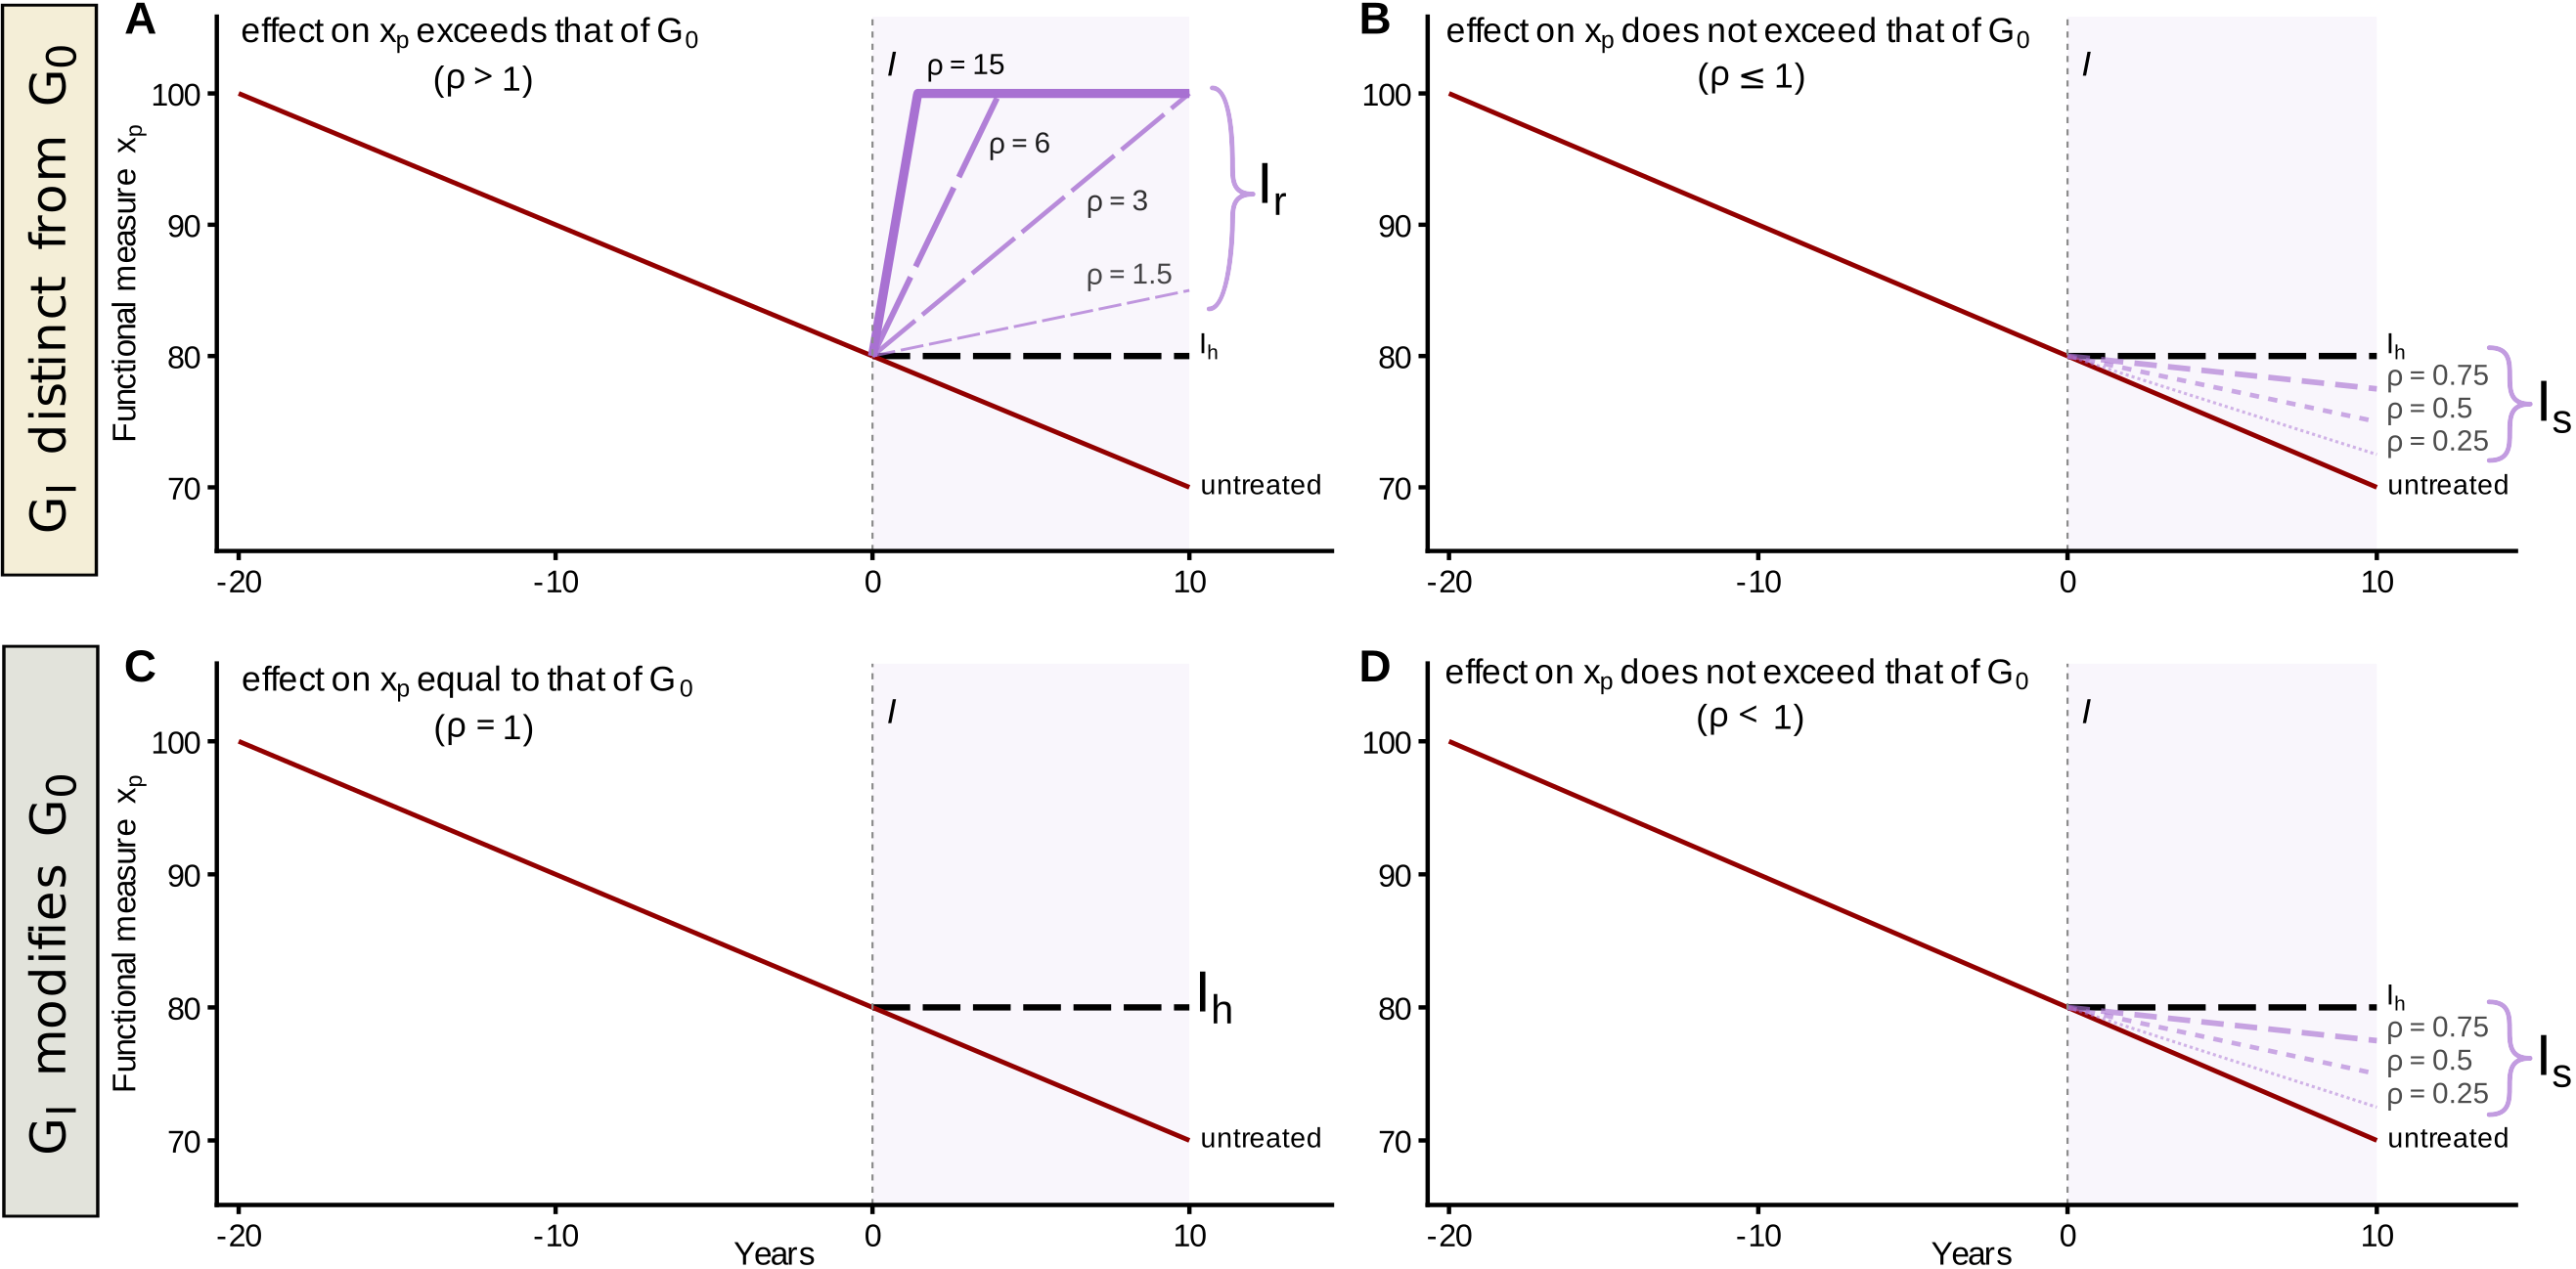
\includegraphics[width=1\linewidth]{figures/Figure_1.png}
	\caption{\textbf{Intervention effects need not share the time scale of the decline they counteract.} Each panel plots a functional measure ($x_p$, e.g.\ handgrip strength) on the $y$-axis against time in years on the $x$-axis, with the intervention applied at year 0 (vertical dashed line, $I$) and the shaded band marking the post-intervention window over which treated and untreated trajectories are compared. The solid dark-red line shows the ``untreated'' trajectory, along which $x_p$ declines under the baseline generative process $G_0$; purple lines show treated trajectories under an intervention, and the black dashed horizontal line marks the trajectory of an intervention that halts further change ($I_h$). Interventions are characterized by $\rho$, the ratio of the magnitude of the intervention's effect on $x_p$ to that of the change produced by $G_0$ over the same interval, which distinguishes three intervention classes: reversal ($I_r$), in which $x_p$ recovers toward its earlier value; halting ($I_h$), in which $x_p$ is held constant; and slowing ($I_s$), in which $x_p$ continues to decline but at a reduced rate. Line opacity and weight scale with $\rho$. Rows correspond to the relationship between the intervention process $G_I$ and the baseline process $G_0$: $G_I$ distinct from $G_0$ (top, \textbf{A--B}), in which the intervention introduces a separate process that counteracts $G_0$, and $G_I$ modifies $G_0$ (bottom, \textbf{C--D}), in which the intervention fine-tunes the parameters of $G_0$ rather than introducing a distinct process. \textbf{(A)} When $G_I$ is distinct and its effect on $x_p$ exceeds that of $G_0$ ($\rho > 1$), the change is reversed ($I_r$), with trajectories shown for $\rho = 1.5, 3, 6,$ and $15$; larger $\rho$ produces faster and more complete reversal. \textbf{(B)} When $G_I$ is distinct but its effect does not exceed that of $G_0$ ($\rho \leq 1$), the decline is slowed ($I_s$), with trajectories shown for $\rho = 0.25, 0.5,$ and $0.75$. \textbf{(C)} When $G_I$ modifies $G_0$ and its effect equals that of $G_0$ ($\rho = 1$), the best attainable outcome is halting the decline ($I_h$); reversal is not possible, as the intervention acts on the process generating the decline rather than restoring prior loss. \textbf{(D)} When $G_I$ modifies $G_0$ and its effect does not exceed that of $G_0$ ($\rho < 1$), the decline is slowed ($I_s$), with trajectories shown for $\rho = 0.25, 0.5,$ and $0.75$. These are simplified scenarios to illustrate the point of when $G_I$ would share a similar time scale to $G_0$.}
	\label{fig:figure_1}
\end{figure*}

\begin{figure*}[!t]
	\centering
	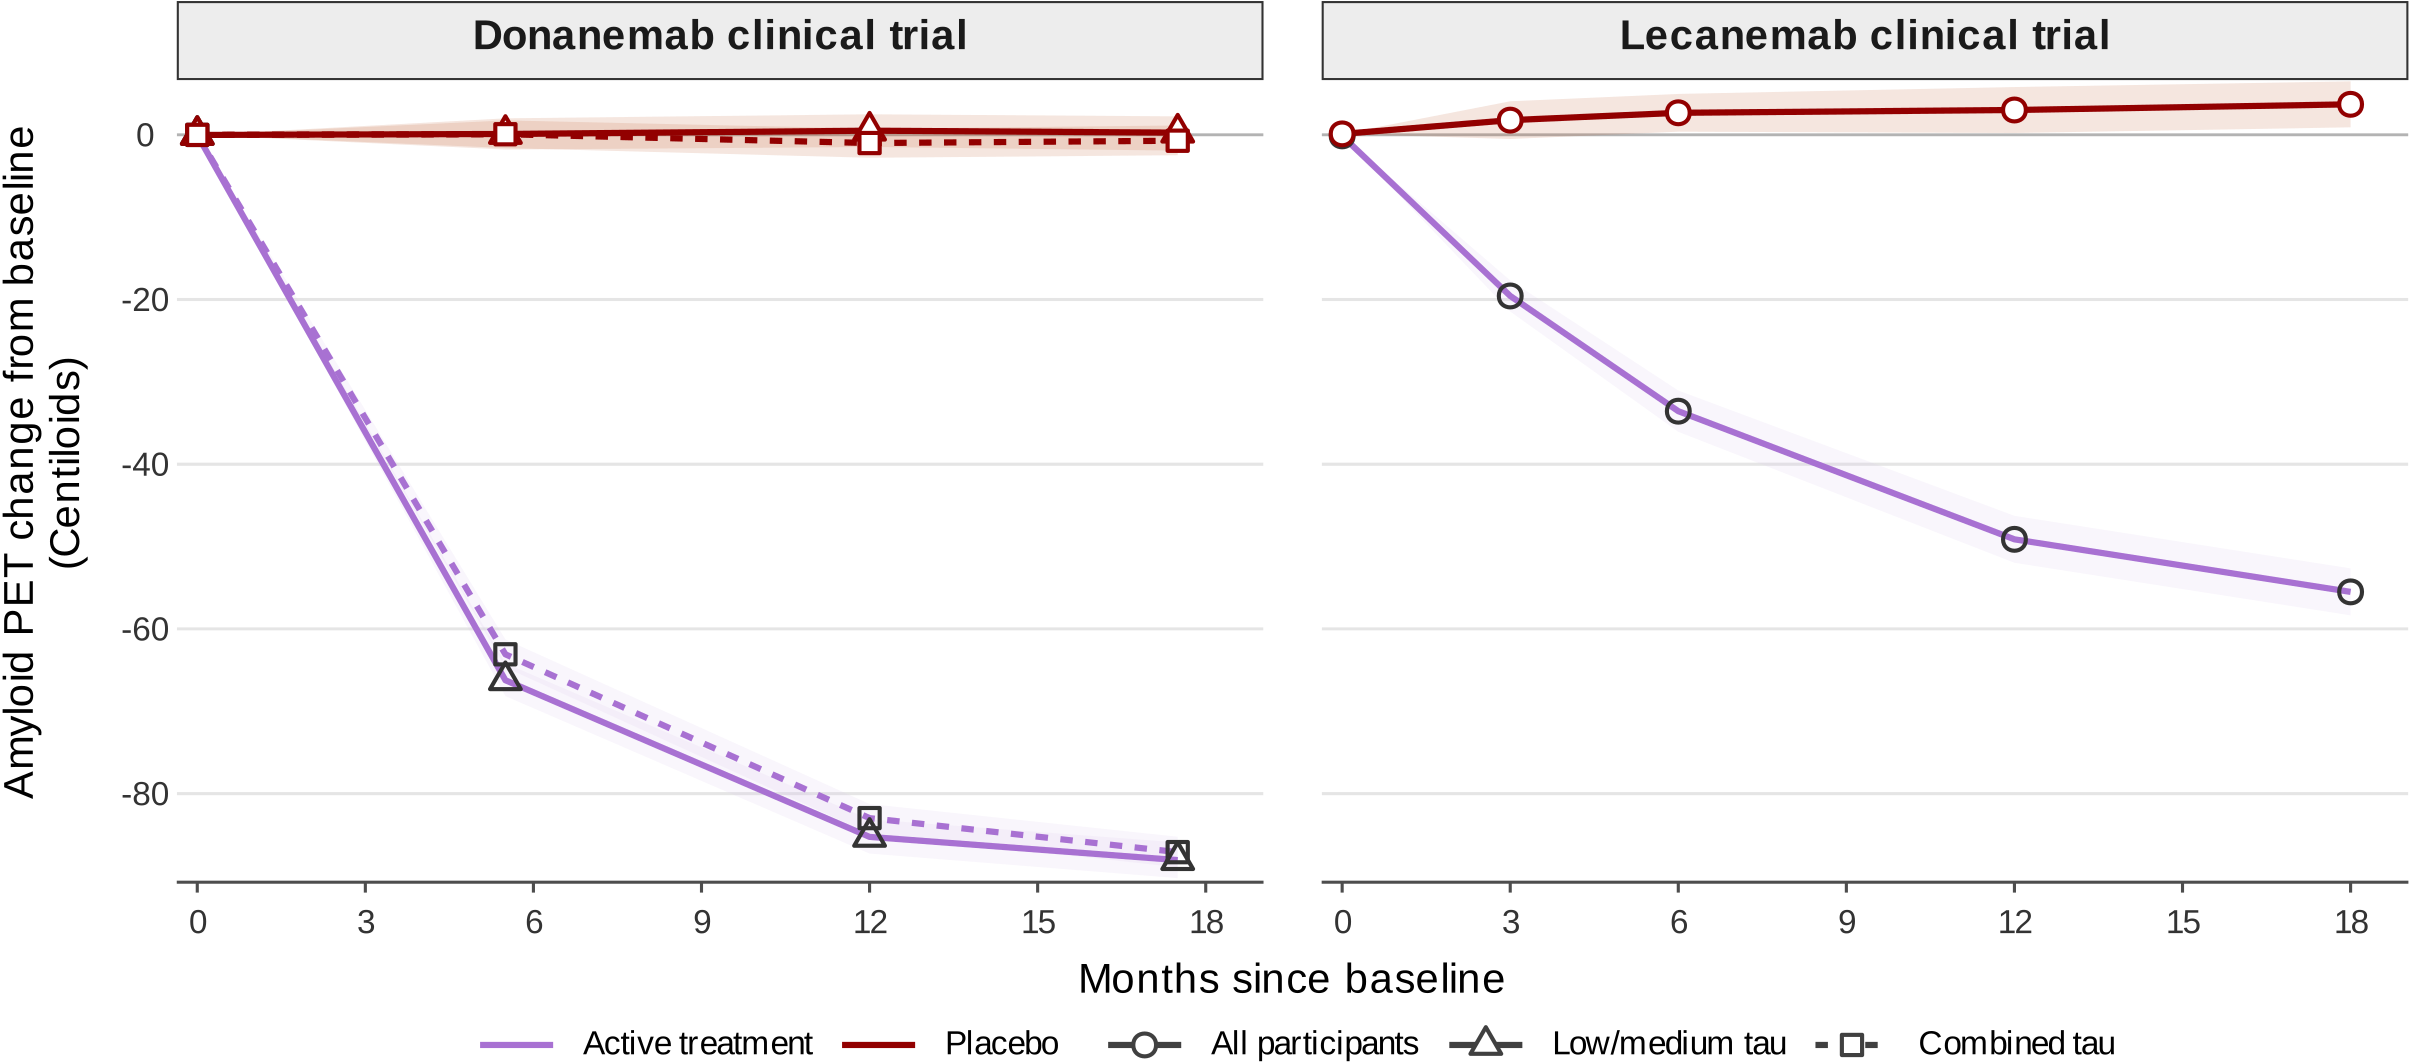
\includegraphics[width=1\linewidth]{figures/Figure_2.png}
	\caption{\textbf{An empirical example in which $G_I$ does not share the time scale of $G_0$.} Each panel plots the adjusted mean change from baseline in amyloid PET signal, in Centiloids, on the $y$-axis against months since baseline (0--18) on the $x$-axis. Panels correspond to two phase 3 anti-amyloid monoclonal antibody trials: donanemab (TRAILBLAZER-ALZ 2, left) and lecanemab (Clarity AD, right). Within each panel, purple lines denote the active-treatment arm and dark-red lines the placebo arm; negative values indicate a reduction in the measure relative to baseline. Point shape and line type denote the analysis population: for donanemab, results are shown separately for the low/medium tau population (triangles, solid) and the combined low/medium-and-high tau population (squares, dashed); for lecanemab, results are for all participants in the PET substudy ($n = 698$). Shaded bands are 95\% confidence intervals; for lecanemab these were derived as $\pm 1.96 \times$ the published standard errors. Values were digitized from Figure 3A of Sims et al.\ (2023) \cite{sims2023donanemab} and Figure 2B of van Dyck et al.\ (2023) \cite{van2023lecanemab}; the figure is adapted from those sources.}
	\label{fig:figure_2}
\end{figure*}


Assumption $A1$ is a composite of two presumptions. First, intervention effects are expected to emerge on a time scale resembling that over which the deterioration originally developed. Second, if effects are small or slow to emerge, increasing sample size, extending follow-up, or both are assumed to be the principal ways to make them detectable.

\subsubsection*{Intervention Time Scales}

The expectation of similar time scales presupposes a particular relationship between the baseline process $G_0$, which produces the age-associated change in a variable $x$, and the process under intervention $G_I$. Yet this represents only a subset of the possible relationships between them, not all of which support this expectation.

When $G_I$ is distinct from $G_0$, it may counteract its effects on $x$ with different temporal dynamics.  At one extreme, deterioration that develops gradually over years under $G_0$ may be partially or fully reversed much more rapidly under $G_I$. Suppose\footnote{Hypothetical scenarios are used throughout the article because simplified, and sometimes extreme, cases can make the logical implications of an argument clearer.} an autologous young heart could be grown for an individual and transplanted. Cardiac function would have taken decades to decline, yet the transplantation restored function over the much shorter time scale of the surgical intervention and recovery. This is not merely hypothetical. Existing interventions that clear age-associated accumulations illustrate the same principle. Antibodies developed against amyloid are one example. In two trials, donanemab and lecanemab substantially reduced mean amyloid PET levels within months (\textbf{Figure~\ref{fig:figure_2}}). The accumulation had taken decades to build under $G_0$; it took months to reverse under $G_I$. The contrast is clear in the placebo groups, where mean amyloid PET levels barely changed over the same 18 months\footnote{An alternative interpretation is that amyloid burden had approached a plateau by this stage \cite{jack2013brain}. This does not affect the comparison. Whether $G_0$ produces slow accumulation or a plateau, the rapid reduction under $G_I$ occurs on a markedly different time scale.}. At the other extreme, a distinct $G_I$ may only partially offset $G_0$, producing slower deterioration rather than reversal. Suppose liver function declines under $G_0$ as dysfunctional hepatocytes accumulate, while $G_I$ selectively eliminates them and allows functional cells to repopulate the tissue. If elimination greatly exceeds accumulation, function may recover rapidly; if it only partially offsets accumulation, decline is merely slowed. Thus, when $G_0$ and $G_I$ are distinct, the time scale of the observed change depends on their relative effects on $x$, rather than being determined by the time scale of deterioration under $G_0$.

The relationship typically presumed by $A1$ is one in which $G_I$ does not introduce a distinct process but instead fine-tunes the parameters of $G_0$. Suppose replication errors accumulate under $G_0$. Their rate depends partly on DNA polymerase fidelity. A small molecule could allosterically increase that fidelity and thereby reduce the rate of new errors, without correcting those already present. If the accumulated errors contribute to functional decline, the intervention slows the process generating that decline rather than introducing a distinct restorative process. Consider the best case for this mode, an intervention that halts new deterioration entirely ($I_h$). The detectable effect is therefore the growing separation between the treated and untreated trajectories. That separation can widen only as $G_0$ continues to generate deterioration in the untreated group. Even in this best case, detectability is therefore limited by the time scale of $G_0$. For an intervention that only slows deterioration ($I_s$), the trajectories separate more slowly still.

\subsubsection*{Detectability by Design}

The second presumption is that small or slowly emerging effects make trials prohibitively costly or impractical. This follows from treating larger samples, longer follow-up, or both as the principal ways to make such effects detectable. These are indeed simple ways to increase detectability\footnote{Larger samples improve the ability to detect small differences between groups, while longer follow-up allows the trajectories under $G_0$ and $G_I$ to diverge further.}, but they are also major contributors to trial cost and duration. The financial cost of a study scales with the number of participants enrolled and the duration over which they must be monitored and retained. 

Sample size and follow-up duration, however, are only two variables within a broader study-design space—the set of variables that define how a study is conducted. The use of molecular measures as surrogates is itself one such design modification: the endpoint is changed under the assumption that molecular features provide an earlier or more sensitive readout of intervention effects. But changing the endpoint is not the only way to alter detectability. The following sections examine alternative design strategies that can improve detectability without relying on molecular surrogate endpoints. These examples are illustrative rather than exhaustive.


\subsubsection*{Study-Design Simulations}

To make the study designs and their implications more intuitive, the observable variable x was taken to be handgrip strength $h$ measured over time $t$. The intervention was assumed to produce a small reduction in the rate of decline ($I_s$). This is the case least favorable to detection and the one most closely aligned with the presumption underlying $A1$. The objective was not to model handgrip in detail, but to compare its detectability across study designs. For each design, several analysis strategies were evaluated. Each design–analysis combination was simulated in 1000 independent trials. Detectability was defined as the proportion of trials in which the intervention effect was detected at the conventional significance threshold of p<0.05. Intuitively, it reflects the size of the intervention-induced divergence between trajectories (signal) relative to the background variation that obscures it.

\textbf{Data-generating process.} Each simulated individual $i$ entered the trial at an age $a_i$ sampled uniformly between 65 and 80 years\footnote{Reflecting realistic recruitment windows in gerontological trials.}. Handgrip strength was generated from four components: their underlying strength, an adjustment for age at trial entry, change over the course of the trial, and background variation around that trajectory. Formally,

$$
h_{i,t} = \alpha_i + \beta_i(a_i - \bar{a}) +
(\beta_i + \delta \cdot \mathbf{1}_{[i \in \mathrm{treat}]})t +
\varepsilon_{i,t}.
$$

In words,
\[
\begin{aligned}
	\text{handgrip} = {}&
	\underbrace{\text{underlying strength}}_{\alpha_i} \\
	&+ \underbrace{\text{entry-age adjustment}}_{\beta_i(a_i-\bar a)} \\
	&+ \underbrace{\text{change during follow-up}}_{(\beta_i+\text{treatment})t} \\
	&+ \underbrace{\text{background variation}}_{\varepsilon_{i,t}}.
\end{aligned}
\]

Between-individual heterogeneity was introduced by allowing both underlying handgrip strength ($\alpha_i$) and rate of change ($\beta_i$) to vary across individuals. Each was assumed to follow a Gaussian distribution around a population mean:

$$\alpha_i \sim \mathcal{N}(\mu_\alpha, \sigma^2_\alpha), \qquad \beta_i \sim \mathcal{N}(\mu_\beta, \sigma^2_\beta)$$

In words, individuals could be stronger or weaker handgrip and decline faster or slower than the population average. For simplicity, these two characteristics were treated as independent. This assumption was consistent with the BLSA data, where individual estimates of strength and rate of change were only weakly correlated (Pearson $r = 0.11$) after centering age at the sample mean, insufficient to justify a more complex joint model given the objectives of the simulation.

\textbf{Parameter calibration.} To keep the simulations empirically grounded, parameters were calibrated from observed data where possible and from published estimates otherwise. The population parameters $\mu_\alpha$, $\sigma_\alpha$, $\mu_\beta$, and $\sigma_\beta$ were estimated from longitudinal handgrip data from males aged 60 years and older in the Baltimore Longitudinal Study of Aging (BLSA). A Bayesian hierarchical model matching the generative structure above was fitted to these data. Age was centered at the sample mean. Posterior means were then used as fixed simulation parameters. Short-term within-individual variability $\sigma$ could not be estimated directly from the BLSA. Repeated measurements were separated by approximately 279 days on average, making it difficult to distinguish short-term variation from genuine changes occurring between visits. We therefore calibrated $\sigma$ using published test–retest studies of handgrip dynamometry in older adults. These report within-session coefficients of variation of approximately 5\% \cite{venegas2022test,nolan2020factors,bohannon2005test}. At a mean handgrip strength of approximately 33 kg, this corresponds to $\sigma \approx 1.65$ kg. A second, more conservative value of $\sigma \approx 3.5$ kg (CV $\approx 10\%$) was taken from the residual variation of the BLSA model.\footnote{This value is larger because the residual captures more than short-term measurement variation. It also includes longer-term within-individual deviations from the assumed trajectory and other variation not explained by the model.} Simulations were therefore run under both values to examine how increased background variation affected detectability within and across study designs.

\textbf{Intervention effect.} The intervention reduced the rate of handgrip decline by shifting the individual slope by $\delta > 0$. The value of $\delta$ was chosen so that, after two years of follow-up, the expected difference between treatment and control corresponded to Cohen's $d \approx 0.2$. In other words, the simulated intervention produced a small effect relative to the natural differences in handgrip between individuals. This represents an effect that is difficult to detect under a conventional trial design.

\textbf{Study designs and analysis strategies.} The same dataset can often be analyzed in different ways. Some analyses use only part of the available information, while others exploit repeated measurements or comparisons within the same individual. These choices can affect detectability even when the study design itself is unchanged. Three study designs were considered:

\begin{itemize}
	\item[-] \textbf{Two-arm between-individual design.} Participants were randomized to treatment and control groups, and handgrip was measured in the dominant hand at each visit. Three analysis strategies were compared: an independent-samples $t$-test at the final time point,\footnote{Uses only the final measurement from each individual. It compares mean handgrip strength between the treatment and control groups at the end of follow-up. Baseline handgrip is not used, so pre-existing differences between individuals are not accounted for.} an independent-samples $t$-test on change from baseline,\footnote{Uses only the first and final handgrip measurements. For each individual, a change score is calculated as the difference between these two measurements. The test then compares the mean change score between the treatment and control groups. This removes pre-existing differences in handgrip between individuals from the comparison. However, it reduces two measurements to a single change score, does not model their measurement variability separately, and ignores any intermediate follow-up measurements.} and a linear mixed model (LMM) testing whether the trajectories of the two groups differed over time.\footnote{Uses all handgrip measurements collected during follow-up. Using these measurements, it estimates the rate of change in handgrip for each individual over time. It then tests whether the average rate of change differs between the treatment and control groups. This makes use of intermediate measurements rather than only the first and last. It also accounts for repeated measurements coming from the same individual.}
	
	\item[-] \textbf{Within-individual split-body design.} This design applies when the intervention is expected to have a local effect. In other words, treating one hand is not expected to affect the other. Each participant received the intervention on the dominant hand, while the non-dominant hand served as the control. The key advantage is that treatment and control are compared within the same individual. Differences between individuals therefore contribute much less to the background variation. Two analysis strategies were compared: a paired t-test on the change scores of the treated and untreated hands,\footnote{Uses the first and final handgrip measurements from both hands. For each individual, the change from baseline is calculated separately for the treated and untreated hand. These two change scores are then compared within the same individual using a paired t-test. The test asks whether, on average, the treated hand changed more than the untreated hand. Because each individual serves as their own control, stable differences between individuals have less influence on the comparison. However, the analysis reduces four measurements to two change scores and does not model the variability of the individual measurements separately. It also ignores any intermediate follow-up measurements.} and an LMM testing whether the rates of change in the treated and untreated hands differed over time.

	\item[-] \textbf{Multi-outcome between-individual design.} This design applies when the intervention is expected to have a systemic effect. In other words, the intervention is expected to affect both hands. Participants were randomized to treatment and control groups as in the standard two-arm design, but both hands were measured at each visit. The key advantage is that the two hands provide correlated measurements of the same intervention effect. Combining them uses more information from each participant and reduces the influence of variation specific to either hand. Two analysis strategies were compared: an independent-samples t-test on the average change score across both hands,\footnote{Uses the first and final handgrip measurements from both hands. For each individual, the change from baseline is calculated separately for the dominant and non-dominant hand. These two change scores are then averaged to give a single overall change score for that individual. The mean overall change is then compared between the treatment and control groups. Averaging across both hands reduces the influence of variation specific to either hand. However, the analysis still reduces the repeated measurements to a single change score and ignores any intermediate follow-up measurements.} and an LMM incorporating both hands and all measurement occasions to test whether the rates of change differed between treatment and control groups.

\end{itemize}

For the latter two designs, non-dominant handgrip was modeled as 10\% lower than dominant handgrip, with individual-level variation of 2 kg (SD), consistent with normative laterality data in older adults \cite{cuyul2025one}\cite{zadon2025analyzing}. The rate of decline was assumed to be the same in both hands. This simplifying assumption was used to illustrate the study-design principles rather than to make claims about bilateral handgrip decline.

For each study design and analysis strategy, sample size, number of measurement occasions, and follow-up duration were varied in turn to examine how each affected detectability. All other design features were held at their default values ($n = 50$, three annual measurements over two years). Sample size ranged from 50 to 200, measurement occasions from 3 to 8 over a fixed two-year follow-up, and follow-up from 2 to 8 years. All simulations were repeated under both values of $σ$ described above.

\subsection{Evaluation of Assumption A2}


Assumption (A2) is also a composite of two claims. First, a molecular variable $x_m$ can stand in for a primary variable $x_p$ in characterizing the effect of an intervention $I$\footnote{Strictly, the primary measure ($x_p$) is not always the final thing we care about. It is usually measured because it helps answer a practical question, denoted here by ($y$). For example, we may care whether an intervention produces enough benefit to justify approval, and use a change in ($x_p$) to make that decision. A surrogate is useful if replacing ($x_p$) with the surrogate leads to the same conclusion about ($y$). Throughout this article, ($x_p$) and ($y$) are treated as effectively interchangeable for simplicity, because the primary measure is usually chosen precisely because it is closely tied to the objective. This need not always be true. A surrogate could predict ($x_p$) well but still fail to answer the question represented by ($y$), or it could be useful for ($y$) without closely reproducing ($x_p$).}. Second, conditional on that validity, $x_m$ provides greater detectability of the intervention effect than $x_p$. These claims are related but distinct. A surrogate may be valid but no easier to detect, or easier to measure but invalid. This section formalizes each claim by specifying the conditions required for it to hold. The substantive evaluation of each is left for the Discussion.

\begin{figure*}[!t]
	\centering
	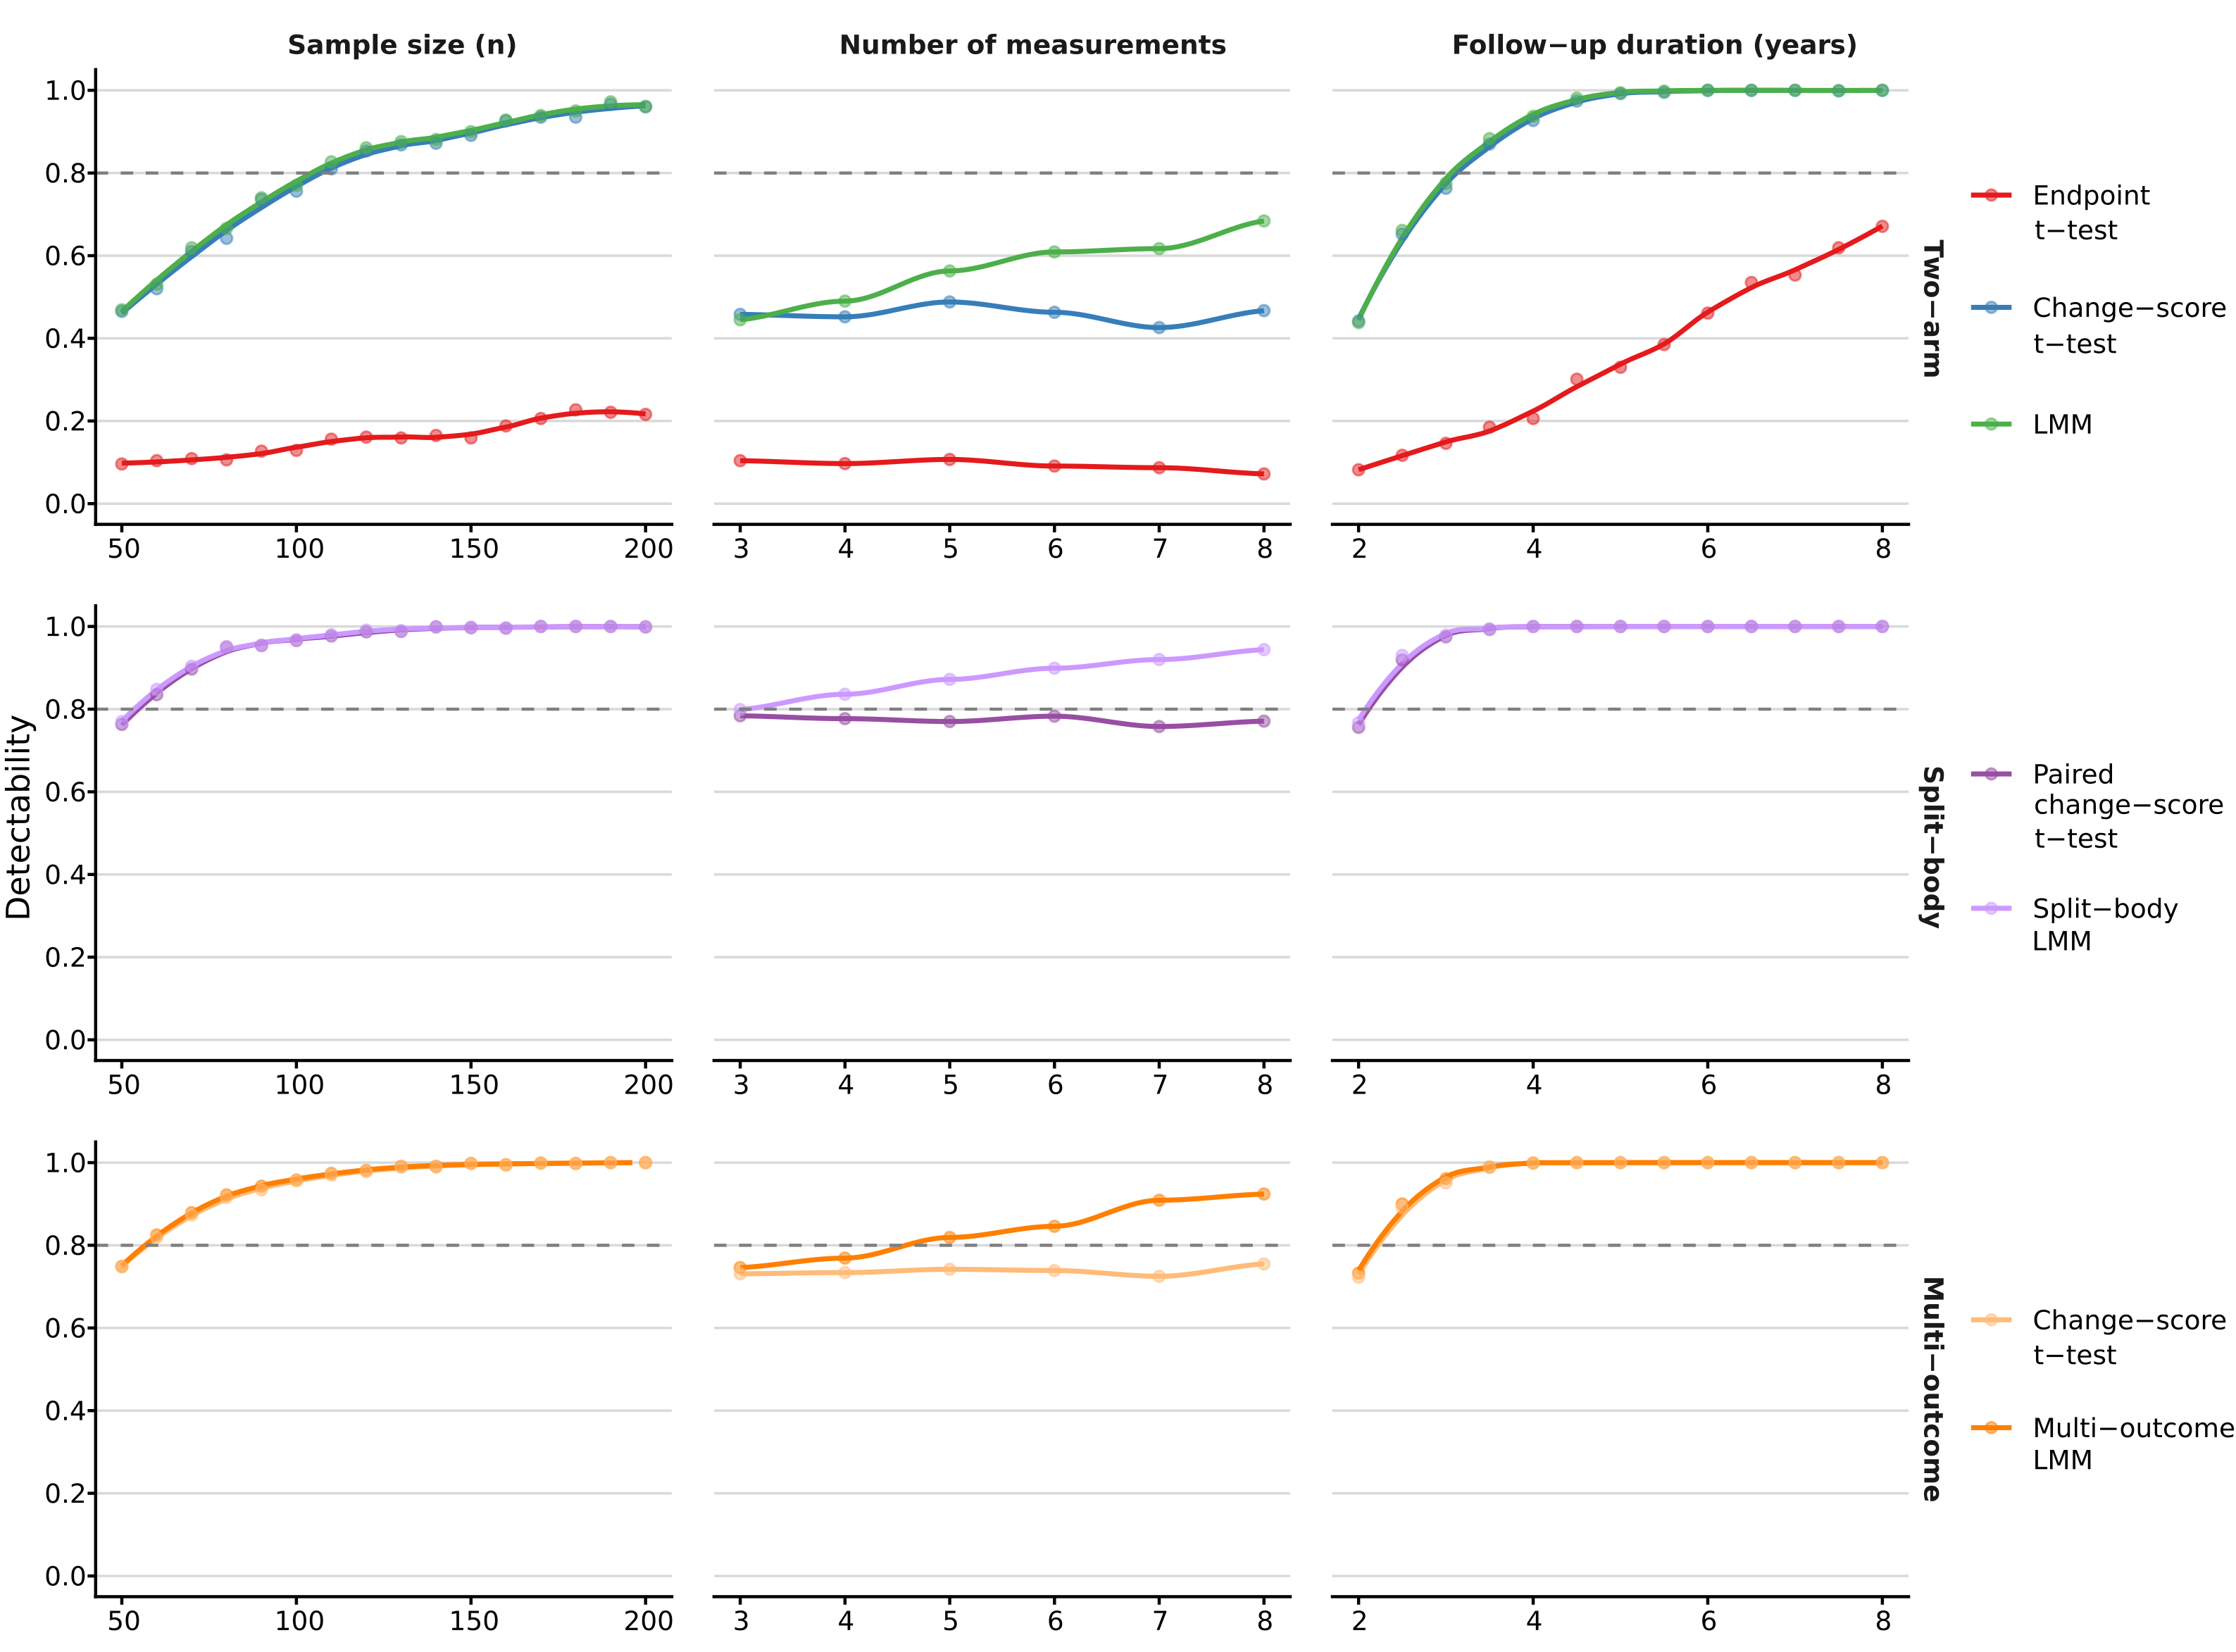
\includegraphics[width=1\linewidth]{figures/Figure_3.png}
	\caption{\textbf{Alternative study designs improve detectability of a small effect without changing the endpoint.} Each panel plots detectability, the proportion of simulated trials in which the intervention effect was detected at the $p < 0.05$ significance threshold, on the $y$-axis against a swept study-design parameter on the $x$-axis. Rows correspond to three study designs: two-arm between-individual (\textbf{top}), within-individual split-body (\textbf{middle}), and multi-outcome between-individual (\textbf{bottom}). Columns correspond to the parameter varied: sample size ($n$, 50--200; \textbf{left}), number of measurement occasions (3--8; \textbf{middle}), and follow-up duration (2--8 years; \textbf{right}). When not being varied, parameters were held at their default values ($n = 50$, three measurements over a two-year follow-up). Within each panel, points represent detectability estimates from individual simulation conditions and lines show the smoothed trend across parameter values. Colors indicate the analysis strategy applied within each design. The horizontal dashed line marks the 0.8 detectability threshold. Each design--analysis combination was simulated in 1000 independent trials. The intervention was modeled as a small reduction in the rate of decline ($I_s$) of a functional measure (handgrip strength), calibrated so that the expected treatment--control difference after two years corresponded to Cohen's $d \approx 0.2$, with within-individual variability set to $\sigma \approx 1.65$ kg.}
	\label{fig:Figure_3}
\end{figure*}

\subsubsection{Validity}

Consider an intervention $I$ that produces, by stipulation, a change in a primary variable $x_p$. A surrogate $x_m$ is valid when a decision made by observing $x_m$ would reach the same conclusion as one made by observing $x_p$. The question is under what structural conditions this holds. Three requirements must be met under the generative process $G_I$ the intervention produces. We label them $R_1$, $R_2$, and $R_3$ for reference in subsequent sections.

\begin{itemize}
	\item[-] \textbf{($R_1$) $I$ produces a change in $x_m$.} A variable that does not respond to the intervention cannot carry information about its effect on anything else, however well-established the relationships of $x_m$ to $x_p$ may be in other contexts.
	
	\item[-] \textbf{($R_2$) $x_m$ is a cause of  $x_p$ under $G_I$.} A variable is a cause of another, if intervening on the first produces a change in the second. A statistical association between the two variables, however robust, is not sufficient. If $x_m$​ and $x_p$​ are coupled because they share an upstream cause rather than because one produces the other, then perturbing $x_m$​ through a route that does not engage the upstream cause will produce a change in $x_m$​ without a corresponding change in $x_p$​.
	
	\item[-] \textbf{($R_3$) $x_m$ fully (or sufficiently) mediates the effect of $I$ on $x_p$.} Every path by which $I$ affects $x_p$ must pass through $x_m$. If any path exists by which $I$ affects $x_p$ without involving $x_m$, then $x_m$ will fail to register intervention effects that nonetheless reach $x_p$.
	
\end{itemize}

The three requirements form a hierarchy. $R_1$ requires only that $I$ changes $x_m$; $R_2$ additionally requires that $x_m$ causes $x_p$ under $G_I$; $R_3$ additionally requires that all effects of $I$ on $x_p$ pass through $x_m$. Each therefore imposes a condition not entailed by the previous one, and the validity of $x_m$ as a surrogate depends on their joint satisfaction. Validity is not an intrinsic property of a measure, but is defined with respect to a particular use \cite{hu2025house, hu2024apples}. Here, that use is the substitution of $x_m$ for $x_p$ in evaluating a specific intervention $I$. Accordingly, the relevant causal structure is that under $G_I$. It need not be the same under $G_0$ or another intervention $G_{I'}$. A surrogate that is valid for one intervention may therefore not be valid for another. The plausibility of these requirements for molecular measures in gerontology is evaluated in the Discussion.

\begin{figure*}[!t]
	\centering
	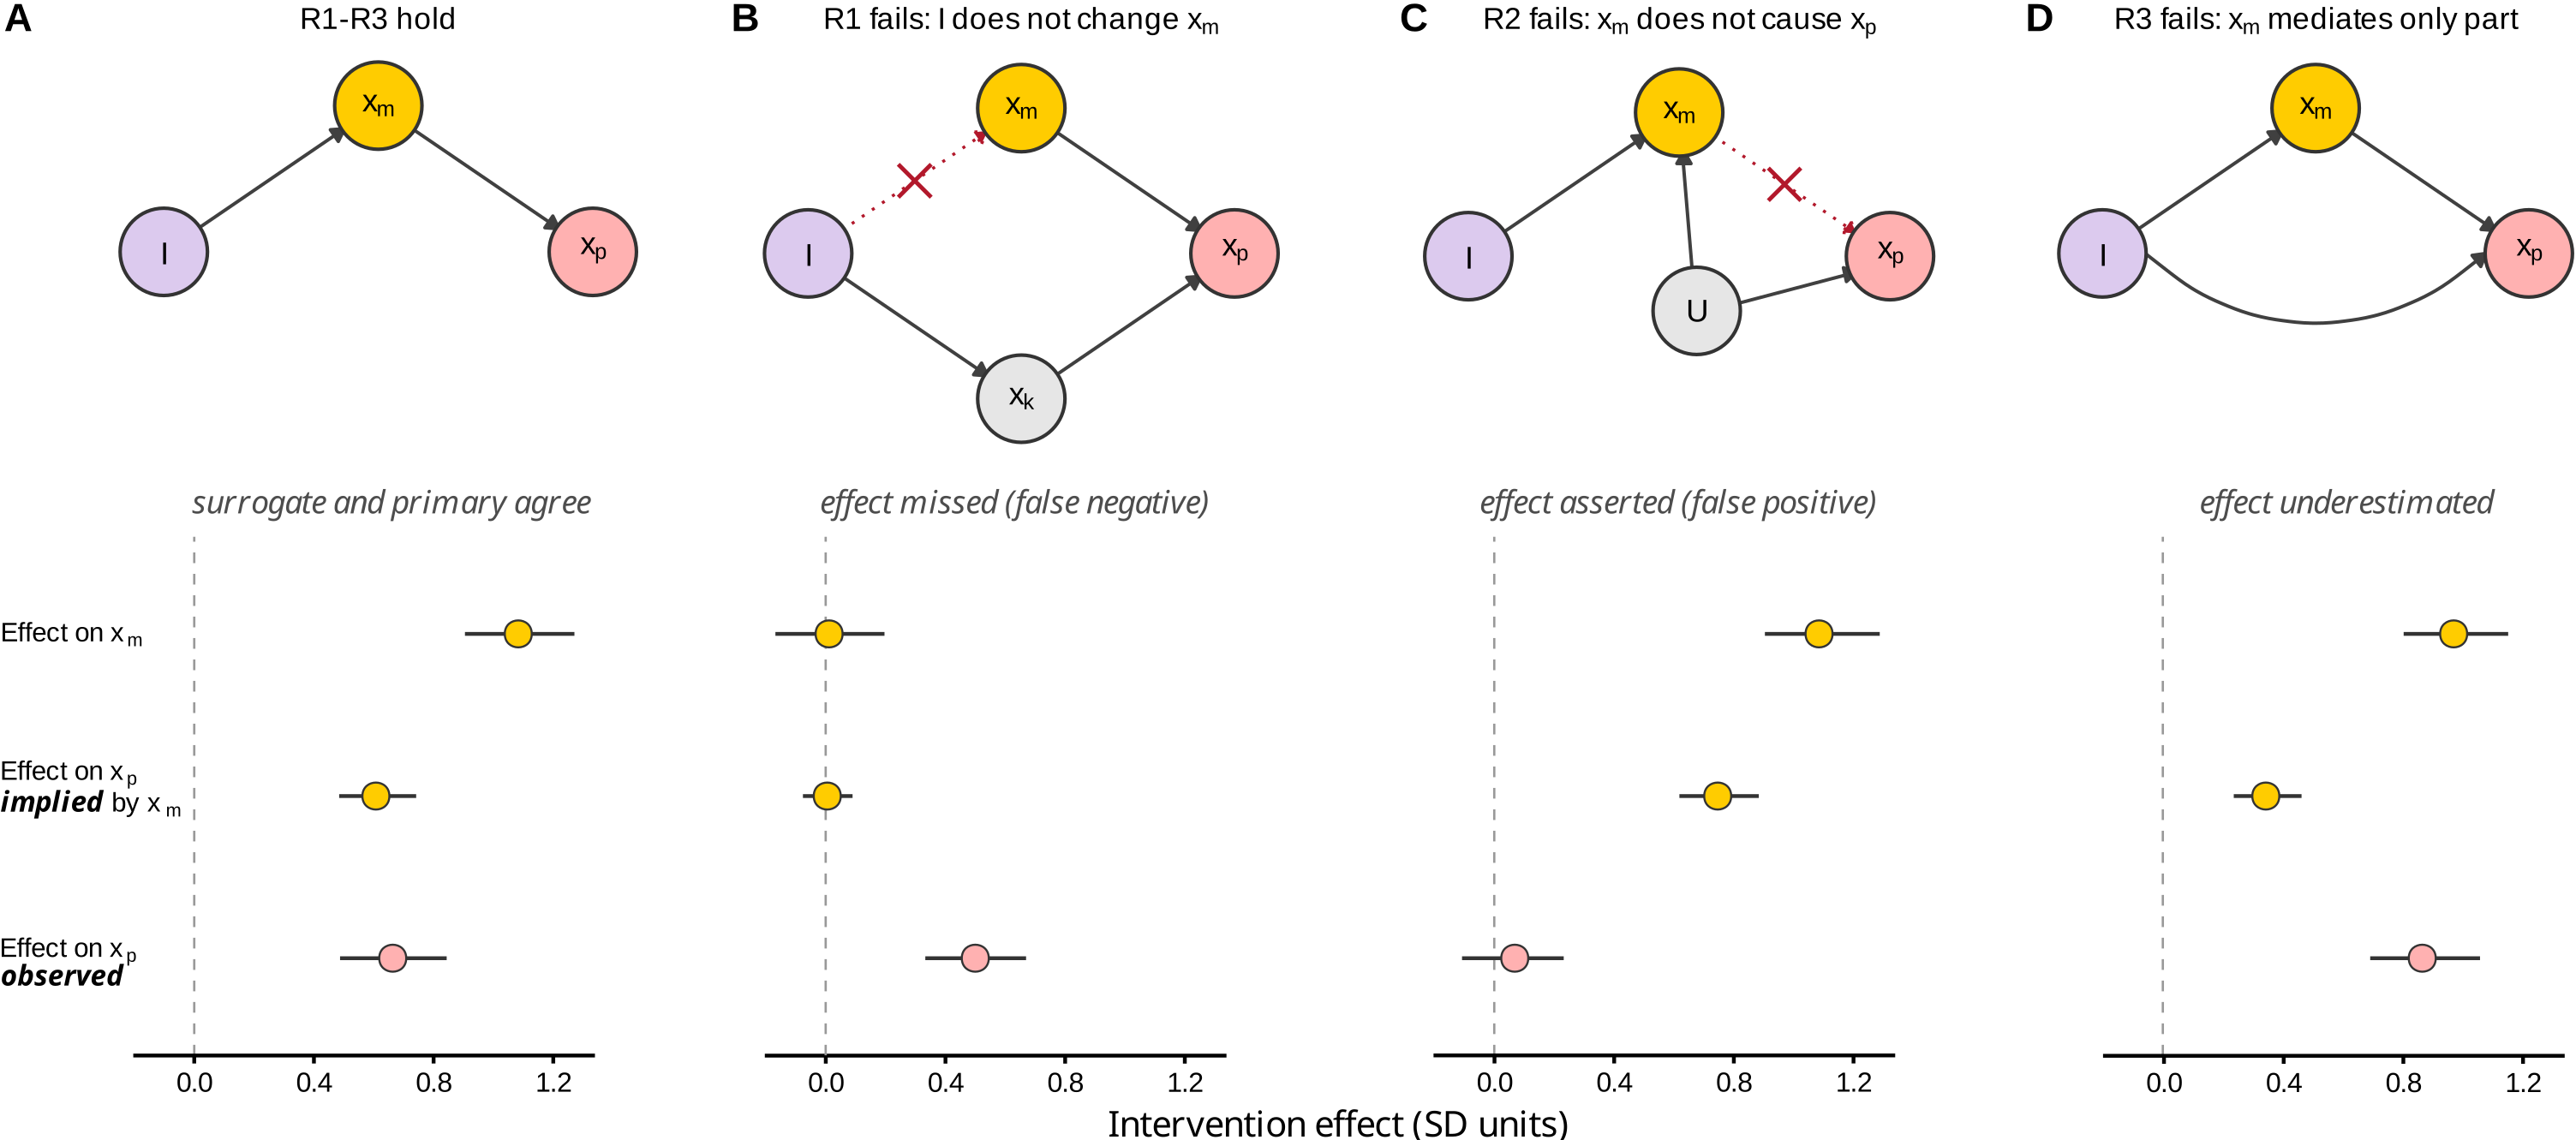
\includegraphics[width=1\linewidth]{figures/Figure_4.png}
	\caption{\textbf{The three requirements for surrogate validity and the consequences of their failure.} Each column pairs a causal diagram (\textbf{top}) with a forest plot of intervention effects (\textbf{bottom}) for one scenario. The diagrams show the causal relationships under the intervention process $G_I$ among the intervention ($I$, purple), the candidate molecular surrogate ($x_m$, yellow), the primary functional outcome ($x_p$, red), and, where relevant, an additional mediator ($x_k$, grey) or a shared upstream cause ($U$, grey); solid arrows denote causal effects, and a red cross marks the absent relationship responsible for the failure. The forest plots show the intervention effect, in standard-deviation units, on the surrogate (effect on $x_m$), the effect on the primary outcome implied by $x_m$ (effect on $x_p$ \textit{implied} by $x_m$), and the effect on the primary outcome actually observed (effect on $x_p$ \textit{observed}); points are estimates and horizontal lines 95\% confidence intervals, with the vertical dashed line at the null (0). \textbf{(A)} All three requirements hold ($R1$: $I$ changes $x_m$; $R2$: $x_m$ causes $x_p$ under $G_I$; $R3$: $x_m$ fully mediates the effect of $I$ on $x_p$): the surrogate and primary outcome agree, and the effect implied by $x_m$ matches the effect observed on $x_p$. \textbf{(B)} $R1$ fails, as $I$ does not change $x_m$ while affecting $x_p$ through a separate path (via $x_k$): the surrogate registers no effect and the intervention effect is missed (false negative). \textbf{(C)} $R2$ fails, as $x_m$ does not cause $x_p$ and the two are associated only through a shared upstream cause $U$: an effect on $x_m$ is asserted where none reaches $x_p$ (false positive). \textbf{(D)} $R3$ fails, as $x_m$ mediates only part of the effect of $I$ on $x_p$, the remainder passing through a direct path: the effect implied by $x_m$ underestimates the effect observed on $x_p$. These are only illustrative instances of each failure; the discrepancy between the implied and observed effect is not fixed in direction or magnitude, and a given failure can leave the surrogate showing no effect, or over- or underestimating the effect on $x_p$ depending on the underlying structure and parameters. Effect estimates are illustrative.}
	\label{fig:Figure_4}
\end{figure*}

\subsubsection{Detectability}

Conditional on validity, $A2$ further assumes that the effect of $I$ can be detected more readily through $x_m$ than through $x_p$. This advantage is often treated as if it followed from $x_m$ being molecular. It does not. It depends on the specific triplet $(I, x_m, x_p)$ and the conditions under which the variables are measured. Greater detectability can arise in several ways. For example, the intervention-induced change in $x_m$ may emerge earlier \citep[f]{waziry2023effect} than that in $x_p$, reducing the required follow-up. It may also be larger relative to the background variation in $x_m$, reducing the number of observations required for detection. In other cases, $x_m$ may simply be easier, cheaper, or less burdensome to measure. These advantages are distinct and need not occur together. These considerations are not examined further here because they depend strongly on the particular surrogate, intervention, outcome, and measurement context. The remainder of the article focuses instead on validity, which must hold before any detectability advantage can justify the use of $x_m$ as a surrogate.

\subsection{Code and data availability}
The code used to generate the simulated data and produce the figures, is available in the GitHub repository associated with this project (link). The BLSA Open Data utilized in this study is available through the Alzheimer’s Disease Data Initiative (ADDI) platform. All analyses and figures were generated in R version 4.4.1. The packages Stan (v2.35.0), ggplot2 (v4.0.3), cowplot (v1.1.3), lmerTest (v3.2-1), and parallel (v4.4.1) and lme4 (v1.1-37) were used for data analysis, handling and visualization. Color palettes were specified using viridis (v0.6.5) and custom manual scales. All figure panels were modified using Inkscape.


%%%%%%%%%%%%%%%%%
% Third Section
%%%%%%%%%%%%%%%%%
\section{Results}

\subsection{Two-arm between-individual design}
Under default conditions (n = 50, 3 timepoints, two-year follow-up), detectability was low in the standard two-arm design across all analysis strategies (\textbf{Figure~\ref{fig:figure_3}, top row}). The unpaired t-test comparing handgrip at the final timepoint showed the lowest detectability (≈0.10). The change-score unpaired t-test and the LMM yielded similar detectability (≈0.45). This reflects the fact that both approaches account for between-individual variability, which constitutes a major component of the total variance. The LMM, despite incorporating all three timepoints, did not substantially outperform the change-score t-test. This likely reflects the magnitude of the change accrued over two years relative to the background variation around each measurement, leaving the third measurement with little to add.

Increasing sample size improved detectability across all three strategies. The unpaired t-test showed only modest gains, with detectability increasing from 0.10 at (n = 50) to 0.22 at (n = 200). In contrast, the two strategies that account for individual variability improved substantially, exceeding 0.8 detectability by n = 110 (0.83 for the LMM and 0.81 for the change-score t-test) and reaching ≈0.96 by n = 200.

Increasing the number of timepoints did not improve detectability for the endpoint or change-score t-tests, as both analyses rely only on the first and last measurements (≈0.43–0.49 for the change-score t-test and ≈0.07–0.11 for the endpoint t-test across the range). In contrast, the LMM, which uses all timepoints to model each individual's trajectory over time, showed improved detectability as more measurements were collected within the same two-year follow-up period. This improvement was modest, increasing from ≈0.45 with three measurements per individual to ≈0.68 with eight measurements, remaining below the 0.8 threshold throughout.

Extending follow-up duration, while keeping the number of measurements (beginning, midpoint, and end) and the sample size unchanged, improved detectability across all three strategies. At the default two-year follow-up, detectability corresponded to that of the default design (≈0.44 for both the LMM and the change-score t-test). The two strategies then improved in parallel, reaching ≈0.77 at three years, crossing the 0.8 threshold shortly thereafter (≈0.88 at 3.5 years), and saturating from five years onwards (≥0.99). In contrast, the endpoint unpaired t-test benefited the least, increasing from 0.08 at two years to 0.46 at six years and 0.67 at eight years.

\subsection{Within-individual split-body design}

Under default conditions (n = 50, 3 timepoints, two-year follow-up), detectability was substantially higher for both analysis strategies compared to the two-arm design (≈0.77 for the paired change-score t-test and ≈0.78 for the split-body LMM, against ≈0.45 for the corresponding two-arm analyses). Achieving comparable detectability in the two-arm design required increasing the sample size to approximately n = 110. The two split-body analysis strategies performed almost identically under these conditions. This improvement arises from the use of within-individual comparisons. By treating the non-dominant hand as a control, between-individual variability in baseline strength and rate of decline is effectively removed. As a result, the noise component is reduced, increasing the signal-to-noise ratio without requiring larger samples or longer follow-up.

Increasing sample size led to a rapid increase in detectability for both strategies. Detectability exceeded 0.8 by n = 60 (0.85 for the LMM and 0.84 for the paired change-score t-test) and reached ≈0.95 by n = 80. At n = 120 both strategies were close to saturation (≈0.99), and both reached 1.00 by n = 170. The two strategies remained closely matched across the entire range, with no appreciable separation between them.

Increasing the number of timepoints did not improve detectability for the paired change-score t-test, as it relies only on the first and last measurements (≈0.76–0.78 across the range). In contrast, the LMM showed improved detectability as more measurements were collected within the same two-year follow-up period.

Extending follow-up duration, while keeping the number of measurements (beginning, midpoint, and end) and the sample size unchanged, led to a rapid increase in detectability for both strategies. Both began at the default-design value of ≈0.76–0.77 at two years, exceeded 0.8 by 2.5 years (≈0.92–0.93), approached saturation by three years (≈0.98), and reached 1.00 by four years.

\subsection{Multi-outcome between-individual design}

Under default conditions (n = 50, 3 timepoints, two-year follow-up), detectability in the multi-outcome design was substantially higher than in the standard two-arm design. Both the multi-outcome change-score and LMM achieved detectability of ≈0.74. This improvement arises from leveraging multiple correlated outcome measures within the same individuals. By jointly modeling these outcomes, the effective signal is amplified while measurement noise is partially averaged out, leading to a higher signal-to-noise ratio compared to single-outcome analyses.

Increasing sample size resulted in rapid gains in detectability for both analysis strategies. Detectability exceeded 0.8 by n = 60 (0.83 for the LMM and 0.82 for the change-score approach) and approached saturation (≥0.99) by n = 130. Compared to the two-arm design, this represents a substantial efficiency gain, as similar detectability levels required considerably larger sample sizes in single-outcome analyses (n = 110 to cross the same threshold).

Increasing the number of timepoints had a modest effect on detectability. As expected, the multi-outcome change-score approach showed little to no improvement, since it relies only on baseline and final measurements (≈0.73–0.76 across the range). In contrast, the multi-outcome LMM, which incorporates all repeated measures across outcomes, showed gradual improvement with additional timepoints. Detectability increased from approximately 0.75 with three measurements to around 0.92 with eight measurements, crossing the 0.8 threshold at five measurements.

Extending follow-up duration produced the steepest gains in detectability. Both strategies began at the default-design value of ≈0.72–0.73 at two years, exceeded the 0.8 threshold by 2.5 years (≈0.89–0.90), reached ≈0.95–0.96 by three years, and were effectively saturated (≥0.99) by four years.

\subsection{Comparison across designs}

Across all conditions, the standard two-arm design required substantially greater resources to achieve the same level of detectability as the alternative designs. Under default conditions, the split-body and multi-outcome designs reached ≈0.72–0.78 detectability while the best two-arm analysis reached ≈0.45. The two-arm design required roughly doubling the sample size (n = 110) or extending follow-up beyond three years. Both alternative designs crossed the 0.8 threshold at n = 60 and before 2.5 years of follow-up, and performed comparably to one another throughout, with the split-body design marginally higher across all three sweeps.

\subsection{Sensitivity to measurement variability}

The qualitative patterns described above were preserved across both levels of within-individual variability (σ ≈ 1.65 kg and σ ≈ 3.5 kg) (\textbf{Figure~\ref{fig:figure_s1}}). Higher variability reduced detectability across all designs but did not alter the relative ordering of designs or analysis strategies. The reduction was nonetheless substantial: under σ ≈ 3.5 kg no design reached the 0.8 threshold under default conditions, and neither the split-body nor the multi-outcome design reached it at n = 200. The threshold was crossed only by extending follow-up, at approximately 4.5 years for the split-body and multi-outcome designs and at approximately 6.5 years for the two-arm design.

%%%%%%%%%%%%%%%%%
% Forth Section
%%%%%%%%%%%%%%%%%
\section{Discussion}

\subsection{Necessity by Design}

Claims that a method is a necessary solution often rely on an implicit framing, making them difficult to evaluate. Making this framing explicit requires three components: the objective, the approaches being considered, and their trade-offs. The promotion of molecular surrogate endpoints assumes that intervention effects unfold on the same timescale as the underlying deterioration, and therefore require large samples, long follow-up, or both to detect.

First, the premise does not apply uniformly across classes of interventions. The assumption that intervention effects unfold on the same timescale as the underlying deterioration depends on the relationship between $G_0$ and $G_I$. It holds only for interventions that modify $G_0$ by halting or slowing it, or that introduce a separate process whose effect does not exceed that of $G_0$. Outside these cases, intervention effects need not follow the timescale of the underlying deterioration or be small or slow to emerge.

Second, even within the class of interventions for which this assumption holds, the alternatives are implicitly restricted. The comparison is framed as one between increasing sample size or follow-up duration and adopting a surrogate endpoint. Study design encompasses a much broader set of choices. Molecular surrogates are themselves one such modification, in which the endpoint is changed under the assumption of earlier or more sensitive detection. Detectability, however, depends on the study design, not only the endpoint. It depends on the ratio of signal to noise, which can be altered through multiple design choices. Increasing follow-up, for example, increases the magnitude of the expected change and therefore the signal. Other design choices act primarily on the noise by reducing irrelevant variance. One common approach is longitudinal comparison, in which individuals are compared with themselves over time. This reduces between-individual variation and better isolates the intervention effect. For interventions that can be applied locally, another part of the same individual can serve as a control. Such designs are common in dermatology. The comparison is then between changes from baseline in the treated and untreated sites within the same individual. This controls not only for baseline differences, but also for shared sources of variability such as systemic factors, measurement conditions, or day-to-day fluctuations. Similar gains can be achieved by exploiting correlations between multiple outcomes. This is particularly intuitive for interventions expected to act systemically. For example, an oral intervention affecting muscle function would be expected to influence both left and right handgrip strength. Observing a small but consistent difference across both measures for the same individual provides stronger evidence than observing the same difference in only one. More generally, collecting multiple correlated outcomes increases the effective information obtained per participant. Although this increases data-collection costs, the marginal cost may be small relative to recruiting and following additional participants. This is especially the case with modern measurement techniques. For example, a single MRI scan can measure muscle volume across multiple body regions. If an intervention has a systemic effect, consistent changes across these regions provide stronger evidence than a change observed in only one.

Third, the feasibility advantage of molecular surrogate endpoints is often misstated. In most cases, approval based on a candidate surrogate endpoint is provisional. It therefore does not remove the need to measure the original outcome. The feasibility being referenced is instead earlier market access, where the product can be sold while the trial is still ongoing, partially offsetting its total cost. The advantage therefore does not arise from reduced measurement or study complexity. If anything, both increase. This distinction is important, as the design options discussed above are not incompatible with molecular surrogates. A surrogate endpoint can be used alongside split-body or multi-outcome designs to improve detectability and reach confirmatory approval earlier.

Taken together, the apparent necessity of molecular surrogate endpoints arises not from an inherent limitation of conventional trials, but from a particular framing of the problem. Once the objective, alternatives, and trade-offs are made explicit, molecular measures become one option among many rather than a required solution.

\subsection{On the Insignificance of Small Effects}

One possible response to the preceding analysis is to dispute the assumptions used in the simulations. Measurement variability may be higher, adherence poorer, or treatment effects smaller than modeled. Any simulation is indeed a manifestation of the assumptions used to construct it. The preceding section, however, took the value of detecting these effects for granted and asked only how they might be detected more efficiently. That premise is worth examining. Every introductory statistics text draws a distinction between statistical and clinical significance. Detecting a small effect more efficiently does not by itself establish that the effect is worth pursuing. An intervention whose benefit is so small that it requires years of sustained exposure before any meaningful difference becomes apparent may have limited practical value to the individual receiving it. Two common defenses are often invoked in response.

The first is an aggregation argument, which holds that individually small effect interventions, once confirmed, could be combined into a substantial additive or synergistic intervention. However, the value of a combination cannot be inferred directly from the value of its components. A combined intervention constitutes its own generative process, with distinct pharmacology, tolerability constraints, interactions \citep{keys2025emerging}, and risks. Interactions between interventions may be additive, sub-additive, synergistic, or antagonistic, might amplify adverse effects, or cause new ones to emerge that are absent from either intervention in isolation. If the combination is claimed to be valuable, that claim requires evidence from the combination itself, not extrapolation from its components. There is also an internal tension in this defense. If a much larger combined effect is expected, this undermines the premise that intervention effects are too small to evaluate without a surrogate.

The second is the compounding argument, which holds that a modest slowing of deterioration can become clinically meaningful if sustained long enough. As with the aggregation defense, this relies on extrapolating beyond the conditions actually tested. A trial conducted over a few years in a specific older population does not support claims about the magnitude of benefit that would accrue over decades \citep[b]{keys2025emerging}, or whether the same effect would hold in younger populations \citep[c]{rolland2023challenges}. Such projections assume that the intervention continues to act with similar magnitude over time, without substantial adaptation, resistance, counter-regulation, or attenuation outside the tested range. A trial conducted over several years in older adults does not by itself establish these claims. As such, the projected long-term benefit is partly a model-based extension rather than an observed result.\footnote{A third defense sometimes invoked shifts the objective from the individual to the population level. First, this is a different objective rather than a response to whether the intervention is meaningful for the individual. Second, the argument is structurally tautological. Almost any small per-individual effect, when multiplied across a sufficiently large population, yields a large aggregate number. If population-scale aggregation is the relevant criterion, then an intervention with a larger per-individual effect would, across the same population, produce an even larger aggregate benefit. The argument therefore does not favor small-effect interventions specifically. It favors whichever intervention has the larger per-individual effect. Finally, population-level projections are typically derived from models whose outputs depend heavily on their assumptions, many of which simplify the underlying biological, behavioral, and demographic processes.}

This highlights a broader asymmetry. Small effects often require ambitious extrapolation to appear important. Their practical relevance is located not primarily in the observed trial result, but in what is assumed to happen beyond it. Yet validating those assumptions may require the very long and complex studies whose impracticality motivated the turn to surrogate endpoints in the first place.\footnote{A related consideration for interventions whose benefits lie far in the future is real-world adherence. Willingness to sustain an intervention tends to decline as the gap between action and perceived benefit widens. This is not specific to gerontology. Smoking provides one example. Its long-term health effects are substantial and well established, yet cessation rates remain modest even among individuals aware of the risks. Exercise and dietary modification provide similar examples. Both have well-established benefits, yet sustained adherence remains low. Addiction, palatability, and other factors also contribute, but the point here concerns the temporal structure of the benefit. Both the cost of an intervention and the tangibility of its benefit affect uptake and sustained use. Small-effect interventions requiring prolonged exposure before any perceptible benefit emerges are unfavorable on both dimensions.} This is not to argue that small effects have no value. Well-characterized small effects may contribute to mechanistic understanding. The issue is one of prioritization under constraint. Time, funding, and personnel are finite. The relevant question is therefore not only whether an effect can be detected, but whether pursuing it is the best use of available resources \citep[c]{keys2025emerging}. Given the scale of gerontological challenges, priority may be better placed on interventions expected to produce larger and more consequential effects.\footnote{The same considerations apply reflexively here. As a self-interested amateur working on these questions, the time available to me is finite. Under these constraints, directing limited resources toward interventions expected to have small effects, and whose confirmation may not arrive within a timeframe I am likely to witness, is not a defensible personal allocation. This is not an argument against others pursuing such work, whose circumstances, incentives, or objectives may differ.}

\subsection{On the Plausibility of Molecular Surrogates}

Even if molecular surrogates are the preferred design option, their use still depends on whether they validly stand in for the primary outcome. Whether a useful mapping can be built between two measures depends on the generative process that links them. Intuitively, the relationship may be harder to model when the measures are far apart in biological scale or time. However, this is only a rule of thumb. A large separation in scale or time can still permit accurate inference: a positive pregnancy test, for example, uses a molecular measure in urine to infer not only a current organism-level state, but also likely changes over the coming months. Conversely, even "nearby" measures may make poor surrogates: a blood pressure reading taken now may poorly predict the reading taken three hours later, because both vary with stress, sleep, caffeine, posture, and measurement conditions. Relative scale, therefore, cannot by itself establish either the promise or the weakness of a candidate surrogate.

As presented in the Methods, three requirements must hold for a surrogate to be valid. $R_1$ requires that the intervention $I$ produces a change in the molecular variable $x_m$. This is usually the simplest requirement to evaluate. One can compare an intervention group to a control group and test whether $x_m$ changes in response to $I$. In practice, $R_1$ often functions as a screening criterion: variables that do not respond to the intervention are excluded as candidate surrogates. Establishing $R_2$ is more demanding. It requires that $x_m$ is a cause of $x_p$ under the generative process induced by the intervention, $G_I$. First, the effect of $x_m$ on $x_p$ may depend on how $x_m$ is modified. Suppose $x_m$ is the abundance of a protein. The same measured increase in $x_m$ could be produced by delivering mRNA encoding the protein, by increasing transcription from the endogenous locus, or by inhibiting degradation of the existing protein. Each may produce the same measured abundance of $x_m$, but not necessarily to the same biological state. The same change in $x_m$ may therefore have different effects on $x_p$ depending on the intervention used to generate it. The causal claim is therefore not simply about $x_m$ in isolation, but about the triplet $(I, x_m, x_p)$.\footnote{This point is related to the broader problem of intervention dependence. The same nominal variable may have different consequences depending on the intervention used to modify it. A related discussion appears in the literature on BMI and intervention-dependent causal effects, as well as in \cite{hu2025house}. The point is noted here only to delimit the issue; it is not the main focus of the present discussion.} Second, even when the causal claim is anchored to a specific intervention, establishing it requires observing $x_p$. This is precisely the measure the surrogate is meant to replace because it is costly, slow, invasive, or otherwise difficult to obtain. A controlled experiment must show that modifying $x_m$ through $I$ produces the expected change in $x_p$. This may be feasible for a specific triplet $(I, x_m, x_p)$, but it cannot be generalized to other interventions without further validation.

The remainder of this discussion focuses primarily on $R_3$, assuming $R_1$ and $R_2$ are satisfied. $R_3$ requires that $x_m$ fully or sufficiently mediates the effect of $I$ on $x_p$. Every relevant path from $I$ to $x_p$ must pass through $x_m$\footnote{Those familiar with "Mendelian randomization" methods may recognize a close analogue to $R_3$. One of its key assumptions is the exclusion restriction, which requires that the genetic instrument affect the outcome only through the exposure of interest, with no alternative paths linking the instrument to the outcome. The extensive debates over this assumption reflect how difficult it is both to establish that no relevant alternative paths exist and to determine when violations are large enough to undermine the resulting conclusions.}. Otherwise, the surrogate will not fully capture the intervention effect. In such cases, the surrogate may fail in either direction, missing effects that reach $x_p$ through other routes or implying a change in $x_p$ that does not occur. As with $R_2$, $R_3$ must be evaluated for a specific $(I, x_m, x_p)$. In principle, $R_3$ could be tested empirically. One could vary the magnitude of the intervention, measure both $x_m$ and $x_p$, and ask whether intervention-induced changes in $x_p$ are captured by changes in $x_m$. If $x_p$ changes when $x_m$ does not, then the intervention must affect $x_p$ through another route. If $x_m$ changes without the expected change in $x_p$, then the observed change in $x_m$ is not sufficient to transmit the effect. However, as with $R_2$, the resulting claim is local. It does not establish that $x_m$ fully mediates the effects of other interventions on $x_p$, in other populations, or under other generative processes. This limits claims that "validated" molecular surrogates would make gerontological trials broadly faster, cheaper, or less dependent on primary outcomes. Such claims require the surrogate to generalize across interventions. If validity remains tied to the tested intervention, the surrogate cannot serve as a general replacement for $x_p$. It can only support an earlier and conditional inference, pending direct evaluation of the primary outcome.\footnote{This is consistent with the earlier discussion of provisional approval. Under current regulatory frameworks, endpoints reasonably likely to predict clinical benefit can support conditional approval, but this does not make them equivalent to the primary clinical outcome. Confirmation still requires measuring the clinical endpoint the surrogate was intended to stand in for.}

Before considering specific examples, it is useful to examine the structure of biological organisms, as this bears directly on the plausibility of $R_3$ for some measures. The configurations biological systems occupy are not arbitrary; they are the result of constraints. Some are structural, such as the elements available in a given environment and their properties. Others arise through selection. Identifying these constraints helps determine what can be inferred about the system. A simple illustration makes this intuitive. Consider the function of "green fluorescence" ($F$), measured by exposing an organism to ultraviolet light and quantifying the emitted light at a defined wavelength. Suppose we observe a population of organisms that share the same level of $F$. Suppose first a structural constraint $C_1$ holds, such that green fluorescence can be produced by only a single protein, GFP1.\footnote{This assumes no other protein structure can emit at the same wavelength. In practice this is unlikely, it is a hypothetical to make the example intuitive.} Under this constraint, $F$ permits a strong inference of the protein involved. If the organism fluoresces, GFP1 must be present and functional. Now suppose $C_1$ does not hold, and the same fluorescence can be produced by GFP1 and GFP2, which differ in sequence and structure but emit at the same wavelength. The inference now weakens. Observing $F$ no longer implies the presence of GFP1. It may be produced by GFP1, GFP2, or through any combination of the two. Two organisms may match in $F$ while differing entirely in the molecular route that produces it. The same problem remains under $C_1$ but at a different level. $C_1$ fixes the protein involved, but not how the observed level of GFP1-mediated fluorescence is achieved. The same $F$ may be reached through a stronger promoter that increases GFP1 transcription, duplication of the GFP1 gene, slower degradation of the GFP1 protein, or a cellular context in which a lower amount of GFP1 produces higher fluorescence. The structural constraint therefore fixes the protein involved but leaves the generative route that produces $F$ unconstrained \citep[a]{tononi1999measures}. Furthermore, whether $C_1$ holds or not, it is important to recognize that the same constraint does not support both directions of inference equally. Even when $C_1$ holds, knowing the organism fluoresces implies GFP1 is present; knowing GFP1 is present does not imply the organism fluoresces. The protein might be mislocalized, the surrounding tissue might absorb the emitted light, or a pigment might mask it. The observed fluorescence depends not only on GFP1 but on everything else that must hold for it to be produced and detected. Now suppose we identify a second constraint, $C_2$: this organism survives only if it maintains a minimum level of $F$. Observing it alive therefore suggests that GFP1 is embedded in a configuration that produces detectable fluorescence. Under $C_1$ and $C_2$ together, the mapping between GFP1 and $F$ becomes tighter in both directions. $F$ implies GFP1 because no other protein can produce the signal. GFP1 becomes informative about $F$ because survival has filtered for configurations in which GFP1 actually produces detectable fluorescence.

Biological organisms have, for the most part, been shaped by selection on organism-level measures: fertility, mobility, resistance to starvation, avoidance of predation, and survival long enough to reproduce. The molecular configurations that realize these properties are therefore often constrained only indirectly \citep[b]{tononi1999measures} \citep[a-b]{weiss2000phenogenetic} \citep[a]{weiss2003evolution}. It can be favored or disfavored only insofar as it alters the measure on which selection acts, or changes the costs, risks, and trade-offs associated with producing it. A system selected in this way is under no constraint to realize a function through a single dedicated route, and may even be favored not to\footnote{A familiar illustration comes from gene-set analyses routinely applied to high-throughput molecular data. Substantially different lists of individual genes can nevertheless "enrich" the same higher-level "biological theme". Historically, however, these methods were not developed explicitly to address biological redundancy or degeneracy. Their stated motivations were largely practical. First, combining small but coordinated changes across many genes could provide greater statistical power than testing each gene separately \cite{mootha2003pgc}. Second, simplifying analyses by reducing the large number of measures to a smaller and more manageable set \citep[a-b]{khatri2012ten}\cite{das2020fifteen}. Third, this was also hoped to help "extract biological meaning" from otherwise difficult-to-interpret lists of genes \citep[c]{khatri2012ten}\cite{zeeberg2003gominer, dennis2003david, beibarth2004gostat, subramanian2005gene}. Even when poor agreement between gene-level results was recognized, it was treated mainly as a limitation of gene-by-gene analysis rather than as evidence of degeneracy in the underlying biological system \cite{hosack2003identifying}\citep[b]{subramanian2005gene}.}. Distributing a function across multiple processes through redundancy, degeneracy\footnote{The terms "redundancy" and "degeneracy" are related but distinct, and the difference bears on the argument. "Redundancy" is used here in the strict sense of identical duplication: multiple copies of the same component performing the same function, as with duplicated genes \cite{tononi1999measures}. "Degeneracy" refers to a kind of functional redundancy without structural identity — different components or routes that can perform a similar function under some conditions while differing under others. The distinction is not as clean as the labels suggest. "Identity" is continuous rather than binary. The labels mark regions of a spectrum rather than discrete categories. Both arrangements share two consequences. The first is resistance to insult: whether through identical copies or dissimilar routes, the presence of more than one element capable of sustaining a function makes that function harder to abolish — by mutation, by targeted attack, or by the loss or damage of any single component. The second, and the more far-reaching, is evolvability. When a function is held by more than one element, no single element bears the full selective burden of maintaining it. One copy or route is thereby freed to vary — to drift, accumulate change, and potentially take on a new role — while another continues to cover the original function, so that novelty can be explored without the existing capability being lost. The implications nonetheless also differ in an informative way. Strictly redundant elements, being identical, share their failure modes: a perturbation that disables one — a toxin, an inhibitor, a condition the mechanism cannot tolerate — disables the others in the same way. Degenerate elements, being structurally dissimilar, might not share failure modes; a perturbation that defeats one route need not defeat the others. The trade-off runs the other way too: redundancy may be easier to manage, since identical elements can be governed by the same control, whereas degenerate routes, being dissimilar, may each require their own. This is itself an instance of the point at issue — every structural arrangement carries its own trade-offs and properties, and which is favored is dictated by the constraints imposed on the system.}, and decentralization can confer several advantages. First, such architectures increase robustness \citep[a]{kitano2004biological}: the function can persist despite mutation, damage, environmental fluctuation, or perturbation of any single route. Second, they increase adaptability: different routes can be recruited as internal or external conditions change. Third, they increase evolvability \citep[c]{tononi1999measures} \citep[b]{kitano2004biological}: because the function is not tied to one indispensable route, components can vary, specialize, or acquire new roles without abolishing the original function. Fourth, they relax the demands placed on any individual component: when reliability is secured at the level of the system, cheaper, noisier, or more error-prone components can be tolerated because their failures need not propagate to the function\footnote{This is a general principle of system design, sometimes termed the "paradox of robustness" — though it ceases to seem paradoxical once considered. The example commonly used to illustrate it is data storage. A single hard drive holding valuable data must be built to high reliability, since its failure is catastrophic and its errors corrupt the data irrecoverably — and such reliability is expensive. Once data is instead distributed redundantly across an array of drives, with a higher-level mechanism reconstructing the contents of any drive that fails, the failure of an individual drive is no longer catastrophic. The reliability demanded of each drive accordingly falls, and the economically favored design shifts toward cheaper, higher-failure-rate components whose errors are absorbed by the system. The same logic operates wherever reliability is secured at the system level: error correction at the top relaxes the performance required at the bottom, and components are permitted — and over evolutionary time, expected — to drift toward sloppier, lower-cost states.}\footnote{In gerontology, molecular imperfection is sometimes invoked as an argument for the inevitability of system-level deterioration. The reasoning is that stochastic molecular behavior and low but non-zero error rates amount to an entropic process that cannot be escaped. However, system-level organization can maintain reliable function despite noisy and imperfect components. Biological systems can tolerate, segregate, repair, replace, or eliminate damaged components, and many such mechanisms are already known. Asymmetric cell division provides a simple example, where damaged material can be preferentially segregated into one daughter cell.}. The full set of advantages is too large to treat here and would require a separate discussion. The point here is narrower. Distributed realization is not merely incidental, but an expected consequence of selection acting on organism-level properties rather than on the preservation of particular molecular routes. This weakens the expectation that a single molecular variable will generally satisfy $R_3$. If an organismal property can be produced through several partially overlapping molecular routes, an intervention may affect $x_p$ without all of its effects passing through $x_m$. Conversely, an intervention may move $x_m$ without moving $x_p$ as the system compensates through other routes. Under such architectures, $x_m$ may still be informative. It may report one route by which $x_p$ can be produced, one state of the system, or one response to a particular intervention. It should not, however, be assumed to completely mediate the intervention effect. Its validity remains local to configurations in which the causal route through $x_m$ is both active and necessary.

This is not to claim that biological organization always favors distributed realization. Centralization can also be favored, but under a different set of constraints. One such constraint is coordination \citep[c]{kitano2004biological}. When several downstream effects must occur together, and partial activation is useless or harmful, a common upstream trigger can be favored over independent ones that could act out of step. A second constraint is controllability. It is closely linked to coordination, but concerns the governance of coordinated change. A state that must be reliably entered, maintained, modulated, and exited is easier to govern when control is concentrated at a few points than when it is dispersed across many. A third constraint is signal pooling. Here a central node is favored not because it coordinates downstream effects, but because it integrates upstream information, collecting many separate inputs and resolving them into a single decision. The cellular decision of whether to divide is a clear case. A cell must weigh nutrient availability, growth signals, the integrity of its DNA, and the length of its telomeres before committing to division. These inputs need not be combined by simple summation. In many cases the decision is conjunctive, where a single unmet condition is enough to block division regardless of the others. Routing the inputs through a common decision point allows them to be resolved into one coherent outcome. Where such a node exists, molecular surrogacy becomes more plausible. If an intervention $I$ acts on a node that is both necessary for the downstream state and the point through which the relevant information passes, then the path from $I$ to $x_p$ may genuinely run through $x_m$​, satisfying $R_3$​.

As such, the plausibility of a molecular surrogate for gerontological interventions can be evaluated by considering the constraints likely to govern the surrogate and primary measures of interest. Most primary measures in gerontology, including lifespan, disease-free survival, mobility, and grip strength, are high-level organismal properties. To the extent that they have been under selection, they are likely to have been selected at the functional level, leaving the molecular routes that realize them comparatively free to vary. In some cases, especially for late-life properties whose consequences occur after reproduction, the selective constraint may be weaker still, or absent altogether. The mapping is loosened further by the fact that many gerontological measures concern deterioration or failure. The space of possible failures is usually broader than the space of preserved function. The same loss of grip strength may arise through muscle atrophy, neural decline, joint pathology, impaired metabolism, or any combination of these. Failure of survival may arise through an even larger range of routes. Furthermore, this multiplicity is not only between individuals. Within an individual, somatic selection can generate heterogeneity across tissues and cell populations. As long as function is preserved, the particular molecular route by which it is preserved need not be the same across tissues, individuals, or time. Finally, many gerontological endpoints compound these problems by being aggregate by construction. "Disease-free survival", "frailty", “mobility,” and “death” group together outcomes with different generative histories under a single measured variable. Together, these features make $R_3$ unlikely to hold for arbitrary gerontological interventions. A single $x_m$ may capture one route to $x_p$ or one response to $I$, but it is unlikely to fully mediate all relevant effects of $I$ on the primary outcome.

\subsection{Alzheimer's and aggregates}

Alzheimer’s disease provides a particularly informative case study. First, decades of public and private investment have produced a large empirical record spanning preclinical studies, longitudinal cohorts, post-mortem studies, and, most importantly, two decades of interventional human data from randomized clinical trials. Second, the problem maps directly onto the surrogacy framework outlined above. The primary outcome, $x_p$, is cognitive decline, an aggregate, failure-defined outcome that unfolds over years. The candidate surrogate, $x_m$, is amyloid-β aggregation, a molecular measure, more accessible than years of cognitive follow-up and situated at what is often assumed to be a "more fundamental" layer \cite{fda_surrogate_endpoints}. Third, the inferential problem is narrower than for broader gerontological measures\footnote{Especially those measures that aim to represent "biological age" or overall "functional state" \cite{vera2025multiomic}\citep[a]{waziry2023effect}\cite{hu2025house}.}. Cognition is one component of the broader multivariate "functional" state. This makes Alzheimer's a comparatively favorable setting in which to evaluate molecular surrogacy.


The historical development of amyloid-β as a candidate surrogate involved a progressive expansion in both the scope and strength of the claims made about it.\footnote{This account necessarily compresses a century of observations, debates, and revisions into a few sentences.} Alzheimer’s 1906 report described a single patient with unusually severe, early-onset dementia whose brain contained plaques and neurofibrillary tangles. Kraepelin subsequently named the condition “Alzheimer’s disease” and distinguished it from ordinary old-age (“senile”) dementia. Similar lesions were observed in senile dementia at roughly the same time, yet the two conditions remained separate. Only later were presenile and senile "forms" argued to reflect the same underlying process and increasingly treated as manifestations of a single disease (Blessed, Tomlinson, and Roth 1968). Attention then shifted from plaques to their molecular composition after amyloid-β was identified as a major constituent \citep[a]{hardy2002amyloid}\citep[a]{salloway2014two}. Subsequent observations, including links involving Down syndrome and familial Alzheimer’s disease \citep[d]{hardy2002amyloid}, motivated the stronger claim that amyloid-β was causal rather than merely associated with the disease. The strongest version of this causal interpretation appeared in the amyloid cascade hypothesis (Hardy \& Higgins 1992; Hardy \& Selkoe 2002) \citep[a]{hardy1992alzheimer}), which placed Aβ deposition at the start of the disease process and treated tangles, neuronal loss, vascular damage, and dementia as downstream consequences.

This "primary cause" interpretation, an instance of the full-mediation requirement $R_3$, was central to amyloid-β's promotion, both as a candidate surrogate and as an intervention target. If Aβ deposition sits upstream of tangles, neuronal loss, vascular damage, and cognitive decline, and all relevant effects pass through it, two things follow. First, monitoring amyloid-β would suffice to infer the state of everything downstream, including cognition. Second, more consequentially, it simplifies intervention. Even if similar levels of amyloid accumulation can arise through different upstream processes \citep[b]{hardy2002amyloid}, those processes need not be targeted individually. One can instead intervene on their proposed common mediator, preventing amyloid accumulation or removing existing deposits with the expectation that the downstream pathology and cognitive decline will also be prevented or reduced. This framing motivated numerous interventions aimed at reducing amyloid levels \citep[c]{hardy2002amyloid}. Some sought to reduce Aβ production by inhibiting the enzymes involved in its generation (β- or γ-secretase) \citep[a]{doody2013phase}; others aimed to prevent its aggregation or accelerate its degradation \citep[a]{egan2018randomized}. A further class used active immunization \citep[a]{gilman2005clinical} or monoclonal antibodies to promote the clearance of different forms of Aβ, including soluble species and deposited plaques.

Prior to intervention, observational evidence showed that the mapping between amyloid and cognition was neither simple nor consistent. A nontrivial fraction of patients with a clinical Alzheimer’s diagnosis had no detectable amyloid, while amyloid deposition was repeatedly observed in cognitively unimpaired older adults \citep[a]{gomez2022lesions} \citep[a]{dickson1992identification} \citep[a]{price1999tangles} \cite{herrup2023not}. The deposit, in other words, can be absent where the outcome is present and abundant where it is not. These discordances motivated explanations based on resilience \citep[b]{gomez2022lesions}, individual thresholds, and additional comorbidities that determine whether amyloid accumulation translates into cognitive decline \citep[c]{gomez2022lesions}. More importantly, they prompted changes in trial design. Later anti-amyloid trials increasingly required confirmed amyloid positivity in addition to cognitive impairment \citep[b]{salloway2014two} \citep[d]{gomez2022lesions} \citep[e]{gomez2022lesions}. This restriction effectively conceded that similar cognitive decline can arise through different generative routes, only some of which involve amyloid, and narrowed enrollment to cases in which the proposed surrogate was at least present.

Interventional results complicated the mapping from amyloid to cognition further. Across several mechanistically distinct approaches, amyloid could be lowered without a consistent effect on cognition. Secretase inhibitors \cite{panza2019bace} — semagacestat \cite{doody2013phase} and avagacestat (γ-secretase), verubecestat \cite{egan2018randomized}, atabecestat, and lanabecestat (BACE1/β-secretase) — all reduced Aβ production. None slowed cognitive decline; several — semagacestat at its higher dose, avagacestat, atabecestat, and lanabecestat — worsened it\footnote{Effects were not uniform in magnitude or timing across compounds, but the direction — reduced Aβ, no cognitive benefit — was consistent across all five.}. Earlier monoclonal antibodies showed the same pattern. Bapineuzumab measurably reduced amyloid accumulation and phospho-tau in APOE ε4 carriers but produced no cognitive benefit in either carriers or noncarriers \cite{salloway2014two}. Solanezumab \cite{doody2014phase} likewise showed no cognitive benefit despite confirmed target engagement\footnote{Solanezumab was designed to bind soluble, monomeric Aβ rather than aggregated plaque, and accordingly showed no change in plaque burden on PET. It did engage its intended target: plasma Aβ rose substantially and was sustained throughout treatment, consistent with the antibody binding and redistributing the peptide from brain to periphery. Despite this confirmed engagement, there was no effect on cognition.}. Aducanumab provided an even sharper example of this discordance \cite{budd2022two, lancet2022lecanemab}. Two nearly identical Phase 3 trials\footnote{The trials were prospectively described as identically designed. In practice, they differed in timing and dosing: ENGAGE began a month before EMERGE, and two mid-trial protocol amendments intended to raise more patients to the full target dose affected a larger share of EMERGE's participants, since EMERGE enrolled more patients after the amendments took effect. The authors invoke this difference to explain why ENGAGE failed where EMERGE succeeded. But the biomarker data sit uneasily with this account: amyloid PET reduction and plasma p-tau reduction were similar in magnitude between the two trials at week 78 — amyloid clearance was only about 16.5\% smaller in ENGAGE than in EMERGE — while the clinical outcomes were not merely smaller in ENGAGE but null, and in the high-dose arm numerically worse than the low-dose arm on the primary endpoint. A dosing shortfall of that size is not an obvious explanation for a difference that large. Whether the true cause was the dosing difference, chance, or something else entirely is disputed.}, both initially halted for futility, later showed large reductions in plaque in both trials, yet a small cognitive benefit in one trial and none in the other. Statistically significant cognitive benefits appeared only with lecanemab and donanemab, and even here the mapping was strikingly asymmetric. Both drugs cleared amyloid almost completely. Donanemab brought roughly 80\% of treated patients below the threshold used to define amyloid positivity \cite{sims2023donanemab}, while lecanemab reduced mean amyloid below the same threshold \cite{van2023lecanemab}. Yet the corresponding cognitive benefit remained comparatively small, on the same order as existing symptomatic drugs\footnote{Symptomatic drugs (e.g. cholinesterase inhibitors) treat the effects of neuronal loss without altering its underlying cause or rate. That amyloid clearance produces a benefit no larger than these is notable precisely because it targets the purported cause rather than the symptom.} \cite{daly2024lecanemab}. Nor was the apparent benefit equally strong across cognitive measures within the same trials: the divergence visible on the primary composite scale was markedly weaker on ADAS-Cog for lecanemab and MMSE for donanemab \citep[d]{daly2024lecanemab}.

Taken together, the Alzheimer's case illustrates the general challenges of establishing a valid molecular surrogate for a gerontological measure. First, the same cognitive decline can be reached through more than one route. Amyloid is neither necessary nor sufficient for it. Second, restricting enrollment to a more homogeneous population of confirmed amyloid-positive patients does not settle the matter because validity is intervention-dependent. The same change in the surrogate, produced through different mechanisms, need not yield the same change in the primary measure. Third, even where a benefit did appear, the mapping between surrogate and endpoint was far from a simple proportional relationship \cite{wallach2024associations, mead2023lecanemab}\citep[b]{lancet2022lecanemab}: near-complete clearance of amyloid corresponded to only a modest slowing of decline. None of this is particular to amyloid-β. It follows from the structure of the outcome itself. Cognition is a high-level, failure-defined trait realizable through several largely independent routes, no single one of which every intervention must traverse.

\subsection{The More the Merrier}

Perhaps no single molecular measure can fully mediate the effect of an intervention on a primary outcome, but a set of measures can. In the fluorescence example, if $F$ can be produced by either GFP1 or GFP2, measuring both proteins may be sufficient to account for both routes. By extension, if an intervention affects $x_p$ through multiple molecular routes, one might try to measure each route. The proposal is therefore that $R_3$ need not be satisfied by a single $x_m$, but by a set $N_s = \{x_{m,1}, \ldots, x_{m,k}\}$. This turns a categorical question into a quantitative one. The problem shifts from whether a surrogate exists to how large the relevant mediating set is likely to be. The size $N_s$ matters because the practical value of the surrogate depends on how many measures are required. A small set may be recoverable; a large one may not.

Whether the set contains one measure or many, the underlying task remains the same. In either case, the goal is to construct a model that maps accessible molecular features to a primary outcome that is difficult, costly, or impossible to observe directly. Model construction can be divided into two broad tasks.\footnote{Framing the problem this way is deliberate. The difficulties that follow are the familiar difficulties of model construction. The earlier discussion of constraints can be read in the same terms.} The first, $T_1$, is to identify the measures that are relevant to the outcome. The second, $T_2$​, is to establish how those measures combine to produce it, thereby approximating the underlying generative process. In practice, the two are interlinked and proceed iteratively. An initial feature set predicts the outcome poorly, motivating a search for further features, a revised model, and so on.

Before considering gerontological endpoints, it is helpful to consider a simpler case. Consider a single yeast cell placed in a defined medium under fixed conditions, with the primary outcome defined as the number of cells present after one day. The goal is to construct a model that predicts this outcome from molecular measures available near the start of the experiment. This is a deliberately favorable case. The organism is unicellular; the horizon is short; the ground truth is cheap and exactly observable, requiring only a plate and a day. Consider $T_1$​ first. A standard way to identify features relevant to an outcome is a knockout screen. Each gene is eliminated in turn and the resulting change in $x_p$ recorded. Here the structure discussed in relation to $R_3$​ reappears. Because the system is degenerate and redundant, a large fraction of single-gene deletions produce no detectable change in growth under standard conditions \cite{edelman2001degeneracy}. The absence of an effect from a single-gene knockout does not establish that the gene is irrelevant to the outcome. It may be one of several routes to the same function, masked by the others. The natural remedy is to delete genes in pairs, but this expands the search space combinatorially, with no principled stopping point that guarantees completeness. That double knockouts reveal interactions absent from singles gives no assurance that triples would not reveal more. One might attempt to direct the search using similarity between components, on the expectation that similar genes share function. But degeneracy is precisely the property that dissimilar components can realize the same function, so similarity-guided search is undermined by the same structure it was meant to circumvent. Identifying the relevant inputs is thus already non-trivial in a single cell under complete gene elimination, before any harder questions concerning regulation rather than presence have been raised.

Now grant that $T_1$ has somehow been solved, and that every gene relevant to growth has been identified. Attention then turns to $T_2$. The question of interest is no longer whether a component is present, but how its level, together with the levels of the others, determines the outcome. A series of difficulties arises, each compounded as features are added. First, the relationship between a feature and the outcome may be nonlinear. A change may have little effect over one range and a large effect beyond a threshold. Second, features interact, so the effect may depends on the values of others, and the number of possible interactions grows far faster than the number of features \citep[a]{domingo2019causes}. Third, the order of changes may matter. Activating one pathway before another need not be equivalent to activating them in reverse. Fourth, the duration of a change may matter as much as its magnitude. Finally, feedback and compensation mean that perturbing one feature can provoke adjustments in others, so that the system observed after a perturbation is not the system that was perturbed. Each of these difficulties expands the experimental space that must be probed to approximate the generative process. Adding features therefore does not simply add measurements. It multiplies the number of configurations, perturbations, and histories that must be observed to construct a reliable model.

All of this, moreover, holds within a single fixed context \citep[b]{domingo2019causes}. Medium, temperature, density, and other environmental variables are held constant, while only the internal state of the cell is allowed to vary. Yet these external variables may matter as much to $x_p$​ as any internal feature, and the same challenges apply. First, identifying the relevant environmental variables is itself a search problem, no less demanding than that for internal features. Second, internal and external variables interact, so the two problems compound. A feature's effect depends on the context in which it is measured, and a knockout screen conducted under one set of conditions need not remain valid under another. The space to be probed is therefore not the internal configurations alone, nor the contexts alone, but their product, and the number of possible contexts is itself open-ended.

Finally, suppose the earlier problems disappear entirely. Every relevant component is known, the state of the cell is measured perfectly, and the rules governing their interactions are fully specified. Even then, two practical constraints remain. The first is computational. Complete knowledge of a system does not imply that its future state can be derived at acceptable cost. Chess provides a familiar example. The position of every piece and the rules governing every move are known exactly. Yet determining the outcome remains computationally difficult that heuristics are used instead of exhaustive calculation. A fully specified generative model can therefore remain computationally intractable. The second constraint is economic. A surrogate model is useful only if applying it is preferable to observing the primary outcome itself. In the yeast example, the primary outcome requires little more than a plate and a day. If generating the prediction costs more than simply observing the outcome, the surrogate has no practical advantage.

As such, the plausibility of a gerontological molecular surrogate set depends on the likely size of $N_s$.\footnote{The yeast case is useful because it grants the measure-more strategy unusually favorable conditions. The system is a single cell, can be systematically perturbed, the context can be fixed, and the endpoint is cheap, direct, and reached in a day. Gerontology removes each of these advantages. The object is a multicellular organism, so the route from molecular state to function can differ across tissues, individuals, and time. The context is neither fixed nor fully observable. The system cannot be exhaustively perturbed. The endpoint is slow and costly to observe, while many molecular measurements are invasive or destructive, limiting the trajectories that can be collected from the same individual over time.} The same constraints that make a single surrogate implausible also determine how large that set might be \citep[d]{rolland2023challenges}. As $N_s$ grows, identifying and validating the full set becomes progressively less plausible. At one extreme are theories in which a small number of circulating factors drive deterioration, such as "pro-ageing" factors that accumulate or "anti-ageing" factors that decline. These imply a relatively small mediating set.\footnote{The appeal of such theories is that, if correct, they simplify both measurement and intervention. They imply a relatively centralized structure in which much of the downstream deterioration is mediated through one or a few upstream factors. Measuring those factors could therefore provide an accessible summary of a much broader downstream state. The same structure would also simplify intervention, because altering the relevant factors could in principle modify many downstream effects at once.} At the other extreme are theories in which deterioration emerges from the combined effects of many weakly constrained processes, none of which contributes much on its own. These imply a much larger mediating set. The constraints discussed in the previous section favor the latter possibility. Selection is weak or absent for many post-reproductive properties and often acts on the level of function rather than on a particular molecular realization. Gerontological outcomes are also frequently defined by failure or aggregate states, both of which can arise through many routes. Together, these features imply that $N_s$ is more likely to be large than small.

\subsection{Genetic Dissection of Complex Traits}

An instructive empirical precedent for this strategy - and for the hope that the relevant set $N_s$ might remain tractable - is the quest to identify the "genetic determinants"\footnote{Whether a trait is “genetically determined” is easily conflated across distinct claims \citep[a]{sarkar1998genetics} \citep[a]{terwilliger2003confounding} \citep[a]{weiss2002goings}. Genes and their products are necessary for the development and maintenance of essentially every organismal trait, but this does not imply that naturally occurring sequence variation in any gene required for the trait will explain variation in the trait itself. A similar conflation is common in gerontology, where a gene knockout that increases or decreases lifespan is sometimes taken to imply that naturally occurring variants in that gene would explain differences in lifespan. Knocking out a structural component may collapse the system without revealing how differences arise within an intact system. Necessity under disruption is therefore not equivalent to explanatory or predictive importance under “natural” variation \citep[a]{arias2023master} \citep[b]{arias2023master}.} of "complex traits"\footnote{The looseness of the terms “complex trait” and “complex disease” warrants caution. They are used broadly in the literature to denote traits whose inheritance departs from simple Mendelian patterns, but the resulting category is neither sharply defined nor biologically uniform. It includes metabolic, autoimmune, and psychiatric disorders, as well as continuously distributed traits such as height and blood pressure \citep[a]{lander1994genetic}. No single genetic architecture should therefore be expected across it: the number of associated loci, the magnitude and distribution of their effects, and their dependence on environmental and population context vary substantially both within and between these groups. The terminology is retained here because it is conventional in the relevant literature, though it is arguably ill-defined and of limited conceptual precision for the kinds of distinctions and arguments made in the present discussion \citep[b]{lander1994genetic}.}. It is a search for genomic predictors, one or more variants, of a trait of interest, often the incidence of a disease. Early successes in Mendelian genetics showed that some traits followed simple and regular patterns of inheritance consistent with discrete inherited factors. Similar patterns were later recognized in rare human diseases. By the end of the twentieth century, family-based linkage studies had mapped the responsible loci for many such diseases, among them Huntington's disease and cystic fibrosis. These successes encouraged the expectation that a similar approach could extend to more "quantitative"\footnote{“Categorical” and “quantitative” are not separate classes of traits. The categorizability of a measure is a matter of degree and resolution. Any measure can be divided into categories; the question is how readily this can be done. The labels reflect agreement among categorizers: give the same distribution to different observers, ask them to divide it into groups, and compare their answers. “Categorical” traits produce higher consensus. In statistical terms, this relates to modality. A clearly bimodal distribution invites a similar split; a single mode does not. “Quantitative” usually refers to unimodal traits, where individuals differ by degree and no "clear" boundary separates them into a small number of types.} traits and to prevalent diseases \citep[a]{visscher2012five} \citep[b]{visscher2012five}, which showed familial resemblance of their own, if to a lesser degree. The extension proved difficult \citep[c]{visscher2012five}. For heart disease, diabetes, autoimmune conditions, and psychiatric disorders, linkage findings were often inconsistent and failed to replicate \citep[a]{pritchard2002allelic} \citep[a]{risch1996future}. A prominent explanation was lack of statistical power\footnote{Other explanations were also proposed, including locus and allelic heterogeneity, environmental confounding, and imperfect \citep[c]{lander1994genetic} or convergent phenotype definitions in which similar clinical outcomes arise from different underlying causes. These issues remained challenges for subsequent association studies.} \citep[a]{manolio2009finding}. The variants underlying these traits were assumed to exert weaker effects than those behind Mendelian disorders, leaving linkage underpowered at achievable sample sizes.

The theoretical basis for this expectation had been established much earlier. In the early twentieth century, it was disputed how such quantitative traits could be explained through Mendelian inheritance \citep[a]{visscher2019ra} \citep[d]{lander1994genetic}. It was unclear how discrete inherited factors could produce the smooth distributions observed for traits such as height and blood pressure. To address this, Fisher and others posited that such a trait is governed not by one or two factors but by a large number, each contributing a small and roughly comparable effect \citep[b]{visscher2019ra}. If these effects combine approximately additively, their sum, together with environmental variation, can produce a continuous and often approximately Gaussian distribution\footnote{The direction of inference warrants emphasis. The infinitesimal model showed how continuous variation could arise under assumptions of numerous small, approximately additive genetic effects and environmental variation. Under these assumptions, it can produce an approximately Gaussian distribution resembling that observed for many quantitative traits. The resemblance does not, however, establish that this is the process that generated the distribution. The same or similar observed distribution may arise from different underlying mechanisms. Observing approximate normality is therefore compatible with the infinitesimal model, but does not by itself confirm its assumptions or identify the underlying causal structure.}. This hypothesized model became known as the infinitesimal model and remains central to quantitative genetics to this day. Taken literally, the model implied a daunting search to identify and disentangle a great many loci, each of minuscule effect. By the close of the twentieth century, however, there was hope that reality would prove more tractable \citep[a]{watson1990human}. A prominent expression of this optimism was the Common Disease–Common Variant (CDCV) hypothesis \citep[a]{lander1996new} \citep[a]{mcclellan2010genetic} \citep[a]{reich2001allelic} \citep[b]{reich2001allelic} \citep[b]{pritchard2002allelic} \citep[b]{manolio2009finding}. It proposed that most common-disease risk might be attributable to common susceptibility alleles at a "modest number of loci", with at least "modest effects"\footnote{What exactly the CDCV hypothesis predicted remains contested \citep[d]{visscher2012five}, partly because its early formulations made few firm quantitative claims about how common risk alleles should be, how many loci should contribute, how large their effects should be, or how much disease risk they should collectively explain. Interpretations ranged from a narrow claim about a "simple allelic spectrum" at particular loci to broader claims about the relationship between disease prevalence and the genome-wide frequency and abundance of susceptibility alleles.}. The argument rested on two key assumptions\footnote{Proponents of the CDCV hypothesis also drew support from a small number of then-prominent reports in which common alleles, most notably APOE ε4, were associated with appreciable disease risk \citep[d]{pritchard2002allelic}. Although these examples were consistent with the hypothesis, other disorders, particularly Mendelian ones, showed extensive allelic heterogeneity, with many independently arising rare mutations and no predominant allele \citep[e]{pritchard2002allelic}. This contrast was attributed to stronger purifying selection against variants causing severe, early-onset disease. Examples could therefore be marshalled on either side, while the small and possibly biased sample of characterized loci provided only a thin basis for a general claim about allelic architecture.}. The first concerned selection. Common-disease susceptibility variants would be weakly selected against if they acted mainly after reproduction or had little effect on reproductive fitness. The second concerned population history. Modern humans descend from a "relatively small" ancestral population. Along with assumptions about mutation rates and mutation–selection equilibrium, it was posited that susceptibility variants common in the ancestral population could remain predominant as the population expanded \citep[c]{pritchard2002allelic}.

The CDCV hypothesis gained prominence\footnote{The optimism surrounding the CDCV hypothesis was not universal. Around the same time, Pritchard used a related population-genetic modelling approach but reached a less favourable conclusion, emphasizing that allelic heterogeneity could leave no single susceptibility variant at high frequency and substantially reduce the power of association mapping \citep[a-b]{pritchard2001rare} \citep[f]{pritchard2002allelic}. The contrast with Reich and Lander arose less from radically different numerical predictions than from differences in assumptions, emphasis, and interpretation.} alongside the achievements of the Human Genome Project and rapid advances in sequencing, genotyping, and genomic data analysis \citep[b]{risch1996future}. Together, denser variant maps, falling costs, larger samples, and association analyses comparing allele frequencies \citep[e]{lander1994genetic} \citep[f]{lander1994genetic} \citep[c]{reich2001allelic} \citep[b]{terwilliger2003confounding} \citep[a]{collins1993new} were expected to provide the power needed to detect the variants it posited. Their identification, in turn, was expected to improve risk prediction, enable earlier intervention, guide treatment, and reveal new therapeutic targets. Over the next two decades, genome-wide association studies identified many reproducible associations, but revealed a structure less tractable than hoped \citep[a]{koch2023clinical} \citep[b]{mcclellan2010genetic} \citep[a]{jakobsdottir2009interpretation} \citep[a]{torkamani2018personal}  \citep[b]{torkamani2018personal} \citep[e]{visscher2012five} \citep[b]{terwilliger2003confounding} \cite{weiss2000many}. For most common traits and diseases, associated variants were individually weak, increasingly numerous, and together explained only a limited share of the estimated inherited variation \citep{c}{manolio2009finding}. Rather than uncovering a "modest number" of loci, GWAS provided growing evidence that extensive polygenicity was the norm for "complex traits" \citep[b]{koch2023clinical} \citep[c]{visscher2019ra}. The gap between expected and actual variance explained by identified variants was reflected in debates over “missing heritability” \citep[a]{wray2013pitfalls}  \citep[a]{crow2011missing} \citep[d]{manolio2009finding}.

This discrepancy prompted various responses. A first route was to build more elaborate genomic models. Chief among these are polygenic risk scores \citep[c]{koch2023clinical} \citep[a]{kullo2026clinical}, which aggregate the small contributions of many variants into a single predictor. These vary widely, both in the number of predictors they include, from a few to many thousands and in some cases every measured variant in the genome \citep[d]{koch2023clinical}, and in their statistical structure and underlying assumptions. Their clinical utility, however, remains disputed \citep[e]{koch2023clinical}. Given their statistical nature and the way they are built, their performance is uneven and population-dependent \citep[f]{koch2023clinical} \citep[c]{torkamani2018personal}, further limited by poor transferability across ancestries, difficulties of calibration and standardization \citep[d]{koch2023clinical} \citep[c]{torkamani2018personal}, and an absence of evidence that acting on a score improves patient outcomes \citep[h]{koch2023clinical}. A second route was to measure more. If common variants left much unexplained, perhaps the remainder lay in what had not yet been measured. This motivated the pursuit of rarer alleles through deeper and higher-resolution sequencing \citep[e-f]{manolio2009finding}, the inclusion of structural variation such as larger deletions, insertions, inversions, and translocations \citep[g]{manolio2009finding}, and the incorporation of further molecular layers beyond sequence, among them DNA methylation, chromatin structure, and the abundances of transcripts, proteins, and non-coding RNAs. A third route was to refine the study design itself in hopes of uncovering subtle associations. Efforts here turned to larger samples \citep[b]{wray2013pitfalls}, better matching of cases and controls to account for background differences \citep[h]{manolio2009finding}, the choice of more or less heterogeneous or different ancestral populations \citep[i]{manolio2009finding}, the control of confounders, and a focus on phenotypes that are more reliably and easily measured. 

The decades-long search for the genetic determinants of complex traits carries several lessons for molecular surrogates in gerontology. First, measurement scale alone establishes neither validity nor utility. Genomic variants occupy the same scale, yet range from highly predictive determinants of Mendelian disorders to weak and context-dependent correlates for common diseases. Success in the former did not justify generalization to the latter. Second, and most fundamentally, the case illustrates the difficulty of inferring organism-level outcomes from lower-level measurements when the underlying generative process is distributed across many components and contexts. The CDCV hypothesis was, in effect, a practical example of “the more the merrier” strategy discussed above. It was a bet that the relevant set $N_s$ would be tractable: a "modest" number of common variants, each of modest effect, that could be combined into a useful predictor. What emerged instead was a large and expanding set of individually weak, context-dependent associations that proved difficult to combine into a valid and useful predictor. Advances in sequencing technologies removed an observational constraint. It did not remove the inferential one. In the terms used earlier, it made candidate inputs easier to observe, but it solved neither $T_1$, identifying which inputs are relevant, nor $T_2$​, establishing how they combine to produce the trait. This difficulty is consistent with the structural considerations discussed above. As selection constrains genomic variation through its functional consequences \citep[a]{weiss2000many} \citep[a-c]{weiss2000phenogenetic} \citep[b]{weiss2003evolution} \cite{weiss2000many}, the resulting relationships can take several forms that complicate both ($T_1$) and ($T_2$). First, the mapping is non-unique in both directions \citep[g-h]{lander1994genetic}. The same trait can be produced by a wide range of genotypes, as some Mendelian disorders show through their extensive allelic heterogeneity \citep[i]{lander1994genetic}. Conversely, a single allele can influence many traits (pleiotropy) \cite{gems1998two}, a consequence of the hierarchical and interconnected organization of organisms. Second, most complex traits are associated with a large and growing number of alleles (polygenicity), each of small effect \citep[a]{schlichting1998phenotypic} \citep[b-c]{weiss2002goings}. Third, the effect of an allele is rarely fixed. It is often contingent on the rest of the genome and on environmental context (epistasis) \citep[c]{terwilliger2003confounding}. The same variant can produce different outcomes on different genetic backgrounds\footnote{What is commonly called the reference genome is a consensus representation. This has consequences for the notion of a genetic “background”. Human populations contain substantially divergent haplotypes. The shift from a single consensus to pangenome references - graphs assembled from many individual haplotypes - was a direct response to this diversity. The combinations of these common alternatives generate a large number of genomic backgrounds. This problem does not disappear within an individual. Somatic mutations arising during development and later life generate genetically distinct clonal lineages, so different cells within the same organism need not share an identical genome \citep[d]{arias2023master}. The background against which a variant acts therefore varies both between individuals and among cells within the same body.} \citep[d]{weiss2000phenogenetic}. Even within the same genetic background, the same gene relocated elsewhere in the genome can behave differently still \citep[a]{claridge1997species}. Fourth\footnote{Further complications include maternal effects \cite{brennecke_epigenetic_2008}, parent-of-origin effects, and mito-nuclear interactions \cite{wallace_selection_1975}, to name a few.}, alleles combine in ways that need not be additive, and their effects are typically probabilistic rather than deterministic, shifting the likelihood of an outcome rather than fixing it \citep[a]{wolf_identical_1997} \citep[a-b]{bale_variable_1997} \citep[c]{weiss2003evolution} \citep[c]{arias2023master}. Finally, compounding these difficulties, the human data available for inference are not a random sample of genotype–phenotype combinations. Natural data are already filtered: numerous layers of selection — at the level of gametes, embryos, and viable organisms — remove many combinations before they can ever be observed \citep[a]{jacob_evolution_1977}. Sequencing can reveal this surviving variation with increasing completeness; it cannot, by measurement alone, reconstruct the generative map that produced it. As such, the statistical models that result are heavily dependent on the context in which they were built. Each extension may recover further signal, but also increases the dimensionality of the model, the data required to fit it, and the conditions under which it must be validated. The result is not a general molecular representation of the trait, but a statistical approximation whose usefulness remains tied to the population, trait, and objective for which it was constructed.


\subsection{On the Molecular Dream}

No scale of measurement is inherently superior. A measure does not become more informative merely because it is taken at a finer, or supposedly more “fundamental”, biological scale. Measures differ in cost, speed, invasiveness, logistical burden, and in how much of the underlying processes they integrate. Every measure preserves some distinctions while collapsing others. Whether the discarded distinctions matter depends on what one is trying to infer.\footnote{Any model is constructed at a particular level of resolution, and the appropriate level depends on the objective. A single system, such as the human body, can be modeled in radically different ways depending on the goal. Designing an elevator may only require coarse descriptors like average height and weight. Modifying a gene might demand a finer resolution, where those same descriptors might be of limited utility. There is no level at which the system is described "as it really is", only levels that are adequate or inadequate to a given question. This is why no measure can be ranked as a better or worse surrogate without first fixing the objective it is meant to serve.} Protein abundance within a cell, for example, could be inferred by modeling transcription initiation, mRNA stability, ribosome loading, translation, degradation, localization, feedback, and their interactions, or estimated from a mass-spectrometry measurement. The latter is not an impoverished representation of the molecular detail beneath it. It is the integrated result of that detail, including processes that have not been identified, measured, or modeled. What it does not allow one to infer is the particular route that produced it.\footnote{The same principle is intuitive at another scale. To determine whether someone speaks English, one could attempt to infer it from the structure and activity of the brain, or simply ask them a question in English and observe the response.}

Lifespan, widely used in gerontology \cite{stroustrup2018measuring}, illustrates both sides of this trade-off. It is valued precisely because it integrates the cumulative consequences of numerous exposures, interventions, physiological processes, and failures over the period of interest. Any benefit, harm, or unforeseen side effect that materially affects survival is, by definition, incorporated into the outcome, including effects investigators did not anticipate or know to measure. Yet the same lifespan can arise through very different generative routes. An intervention that extends life, for example, need not preserve mobility, cognition, strength, or other aspects of function. It is this limitation that has motivated decades of debate over the adequacy of lifespan for characterizing gerontological interventions. As such, even if lifespan could be observed immediately and at no cost in human trials, it would still be insufficient. Functional outcomes would still need to be measured. For these outcomes, intervention effects need not be slow to emerge. Even when effects are small or slow, surrogate endpoints are only one way to improve detectability. Even when a surrogate is preferred, molecular measures are unlikely to be the most valid choice, let alone the only one. This is especially the case for measures such as lifespan or functional deterioration. For outcomes that are weakly constrained by selection, late-life, failure-defined, or aggregate, a small and manageable molecular surrogate set is unlikely. Still less likely is one whose validity generalizes across interventions. Expecting this difficulty to be overcome simply by measuring more molecular variables, constructing increasingly elaborate composites, or devoting further effort to making those composites “causal” \cite{teschendorff2025epigenetic} is unlikely to be fruitful in the near term. A more tractable strategy may instead be to use the integrated measures biological systems already produce at many scales, rather than attempting to reconstruct them from increasingly detailed molecular measurements.

New technologies often pass through a familiar sequence \citep[a]{manhart1992molecular}. An initial period of rapid adoption is accompanied by broad optimism about the problems the technology might solve; this is followed by a slower period of consolidation in which its valid uses and limitations are worked out. Molecular measures in gerontology appear still to carry much of the optimism of the former stage. Yet such optimism is difficult to reconcile with what is already known. Within gerontology, the relevant organism-level outcomes arise from heterogeneous, interacting, and partially redundant and degenerate processes, making broad intervention-independent molecular surrogacy an unusually demanding objective. Outside gerontology, closely related ambitions have already been pursued in fields including genomics and molecular systematics \citep[c]{manhart1992molecular}, where increasing molecular resolution repeatedly proved insufficient to eliminate the underlying inferential problem. The difficulty, therefore, is neither unexpected nor unprecedented. Continuing to treat finer molecular measurement and modeling as though they are on the verge of overcoming it risks spending another generation rediscovering limitations for which there is already substantial reason to expect.


%%%%%%%%%%%%%%%%%%
% Appendix Section
%%%%%%%%%%%%%%%%%%
\section{Appendix}

\subsection{Molecular Targets in Oncology}
Oncology provides one of the clearest empirical settings for examining how selection on a trait relates to the molecular routes that realize it, and when molecularly targeted interventions are most useful. At its core, the problem can be framed as one of classification: the aim is to selectively eliminate "cancerous" cells while leaving "non-cancerous" cells unaffected\footnote{Senolytics pursue a structurally similar objective \cite{passanisi2026replicative}. They aim to eliminate a subset of cells from the body in pursuit of long-term health outcomes. Decades of oncology therefore provide an empirical precedent for both the promise of molecular targeting and the conditions under which it is likely to succeed.}. A wide range of approaches have been developed\footnote{Molecular targeting is only one class of oncological intervention. Other successful approaches include surgical resection and radiotherapy for localized disease, as well as cytotoxic chemotherapy. Some cancers are remarkably sensitive to the latter such as testicular germ-cell tumors and low-risk gestational trophoblastic neoplasia.}, most of which attempt to identify a trait that is more prevalent in tumor cells than in the rest of the body. Early chemotherapies, for example, used proliferation as the targeting rule. Many tumor cells divide frequently, so drugs that disrupt DNA replication or mitosis affect them disproportionately. This trait, however, is far from tumor-specific. Many normal cell populations, including bone marrow, intestinal epithelium, hair follicles, and skin, also divide rapidly and are affected accordingly. The well-known side effects of chemotherapy are direct expressions of this limited specificity. The objective has been to refine the targeting rule to capture as many "cancer" cells as possible while sparing "normal" cells.\footnote{This classification problem is difficult for several reasons. First, tumor cells originate from the host. They are built from the same molecular repertoire as the rest of the body and depend on much of the same machinery. Second, tumorigenesis is heterogeneous, both within and across individuals. The mutations, pathways, and configurations that produce a tumor cell are not uniform. Many distinct molecular routes can lead to comparable cellular behavior. Third, what is meant by a "tumor cell" is itself worth making explicit. A cell is labeled tumorigenic if, left in place, it would contribute to the formation of a mass capable of harming the individual. This is a behavioral rather than molecular definition, and the same behavior can arise through many configurations, including overactivation of growth-promoting genes, loss of growth-suppressing ones, metabolic rewiring, and evasion of programmed cell death. Mammalian cells are substantially degenerate, and no single molecular component is universally essential to the tumorigenic phenotype. Finally, the intervention itself changes the population being targeted. Any targeting rule imposes selection on the targeted feature. By eliminating cells that satisfy the rule, the intervention enriches for cells that do not. If even a small subpopulation lacks the target through pre-existing heterogeneity, reduced expression, or alternative configurations that achieve the same function, that subpopulation is more likely to survive and expand.}

The appeal of molecular measures followed directly from this aim. Such measurements might yield better targeting rules than "broader" traits such as proliferation \cite{proctor1995cancer}. The general approach takes a recurring shape. Tumor and non-tumor cells are compared across many measures, typically genomic, transcriptomic, and proteomic, to identify features that are enriched, mutated, or otherwise distinctive in the tumor. A construct is then built to act on this target. The feature may serve simply as a localization rule. An antibody, ligand, or small molecule binds the target and delivers a destructive payload, such as a toxin, radionuclide, or immune effector. Alternatively, if the target is functionally important to the cancer cell, small-molecule or antibody inhibitors are used to disrupt it. The two strategies can also be combined, with a single agent serving as both targeting moiety and modulator.

The ideal scenario would be a trait present in every tumor cell, absent from every normal cell, necessary for the malignancy, and one whose loss the tumor cells cannot readily bypass. Chronic myeloid leukemia (CML) approaches this ideal.\footnote{CML lies near one extreme of a broader spectrum. Other successful molecular targets are shared less uniformly, are less uniquely tied to the malignant state, or produce less complete responses when targeted. Examples include PML--RARA in acute promyelocytic leukemia, CD20 in B-cell lymphomas, CD19 in B-cell leukemias and lymphomas, and HER2 in HER2-positive breast cancer. Their effectiveness varies with how consistently the target is present, how strongly the malignant cells depend on it, whether normal cells also express it, and how readily the cancer can escape its loss.} It is defined by a reciprocal translocation between chromosomes 9 and 22, the Philadelphia chromosome. This feature is so consistent across cases that it was identified in 1960 from gross chromosome morphology and staining alone \cite{nowell1960minute}. Although initially interpreted as a deletion of chromosome 22, it was shown in 1973, with improved staining, to result from a reciprocal translocation with chromosome 9 \citep[a]{nowell1960minute}. Over the following decade, this rearrangement was found to join part of BCR to part of ABL1, forming a fusion gene that encodes a constitutively active tyrosine kinase. Its sufficiency to drive disease was shown when murine bone-marrow cells engineered to express BCR–ABL1 produced a CML-like disease after transplantation into mice \citep[a]{pane1996neutrophilic}. This prompted a search for selective inhibitors. In 1996, imatinib\footnote{The compound was not yet called imatinib in the 1996 study; that name was adopted later.} was shown to inhibit the proliferation and tumor formation of BCR–ABL1-expressing cells. In colony-forming assays, it reduced CML-derived colonies by 92–98\% while largely sparing normal cells \cite{druker1996effects}. Five years later, imatinib received accelerated approval for the treatment of CML. When administered during the chronic phase, imatinib brings life expectancy close to that of the general population. Patients diagnosed today lose, on average, fewer than three life-years to the disease, an outcome rarely achieved in cancer \cite{wedelin1986clinical, bower2016life, druker2025imatinib}.

CML also illustrates the conditions under which the same treatment becomes less effective. The longer the disease is left untreated, the less likely imatinib is to produce a durable response; this is most evident after progression to blast phase, where responses are poorer and relapse is more common \cite{weisberg2007second, druker2025imatinib}. This is thought to result from adaptations acquired by subsets of the malignant cells. Some reduce the effectiveness of imatinib, through mutations in the kinase domain \citep[b]{weisberg2007second}\citep[c]{druker2025imatinib}, increased expression, or amplification of the fusion gene \cite{hochhaus2004clinical, volpe2009imatinib}. Others provide alternative routes for proliferation and survival less dependent on BCR–ABL1.\footnote{CML provides another example of the "more the merrier" approach. One response to resistance is to widen target coverage, either by combining agents or by developing a single agent active against several relevant variants or targets. Ponatinib was designed to inhibit both native and mutant BCR--ABL1, including the T315I variant that confers resistance to earlier inhibitors, and also inhibits several other kinases. It restored responses in many heavily pretreated patients, including those with T315I disease. This broader activity, however, came with substantial toxicity. Serious arterial occlusive events emerged after approval. The toxicity was severe enough that the drug was temporarily withdrawn in 2013 and returned only with a boxed warning and a narrowed indication. Broad kinase inhibition has been proposed as one contributor to this toxicity. Ponatinib therefore illustrates a potential trade-off of increasing target coverage. Doing so may reduce some routes to resistance, while also increasing the number of normal processes affected by the intervention.} Furthermore, treatment selectively eliminates susceptible cells. As such, the malignant state becomes progressively less tied to the molecular feature that initially made it tractable. This erosion of target dependence over time reflects a more general problem. The mapping between a malignant trait and its molecular realization is rarely one-to-one. CML is only one form of leukemia, accounting for approximately 15\% of adult cases \cite{granatowicz2015overview}. Leukemia is defined at the level of the trait, as the malignant proliferation of blood-forming cells. Given the range of presentations grouped under this label, it is unsurprising that there are many ways to reach it. BCR–ABL1 is one such route. Other leukemias arise through different alterations and do not depend on it \citep[b]{pane1996neutrophilic}. Even within CML, the mapping is not unique \citep[c]{weisberg2007second}. Depending on the location of the breakpoint in \textit{BCR}, the translocation can produce the p190, p210, or p230 fusion proteins, which differ in structure, activity, and disease association \citep[a]{lugo1990tyrosine}\citep[c]{pane1996neutrophilic}. The converse also holds: some CML-like features can be produced by other activated tyrosine kinases \citep[b]{wedelin1986clinical}\cite{scott1991v}\cite{daley1990induction}\cite{kelliher1990induction}.

This same pattern is visible across oncology more broadly. Some of the clearest oncological successes occur when intervention acts before substantial heterogeneity has emerged \citep[b]{druker2025imatinib}. Vaccination against HPV or hepatitis B, for example, acts before divergent malignant populations have arisen \cite{kao2015hepatitis}. Gastric MALT lymphoma provides another example. In early H. pylori-positive disease, eradication of the bacterium alone can cause lymphoma regression \cite{bayerdorffer1995regression}. It becomes less effective as the disease progresses and growth becomes less dependent on the initiating infection.\footnote{These cases also illustrate how a common initiating cause need not produce a common molecular cancer state. The same virus or bacterium can give rise to malignancy through different combinations of subsequent cellular changes.}

\subsection{Taxonomic Molecular Dreams}

Structurally similar problems in other fields can be useful guides. First, similar problems may have appeared elsewhere earlier, allowing one to learn from how the debate unfolded, which mistakes happened, and which solutions proved practical. Second, a different contextual framing of the same problem can make its implicit assumptions easier to identify and the structure more intuitive to reason about. The hope that molecular measures can provide practical substitutes for difficult organismal measures and resolve definitional disputes is not unique to gerontology. Taxonomy has had centuries-long debates over how species should be defined \cite{kunz2013species, simpson1945principles} \citep[e]{claridge1997species} and which measurements should be used to distinguish them \citep[c]{kunz2013species}. Many theoretical and operational definitions have been proposed, each privileging different features of organisms. Some emphasize reproductive compatibility, others morphology or ecology. Each came with practical and interpretive difficulties. With the rise of genomic and other molecular measures, a twofold hope emerged. First, established but difficult organism-level measurements could be replaced by more accessible molecular ones. Second, long-standing classificatory disputes could be resolved by moving classification to a more "fundamental" level of measurement.

A popular and widely used definition treats two groups as distinct species if they cannot interbreed and produce viable, fertile offspring. This criterion is often difficult to measure. Testing reproductive compatibility requires controlled crosses, appropriate conditions, and organisms that can actually be bred and followed. In many cases — extinct lineages, geographically separated populations, organisms with long generation times, or organisms whose reproductive conditions are poorly understood — the test is costly and sometimes impossible. A central aim therefore became to identify whether some genomic measure could reliably predict reproductive isolation, allowing it to serve as a species criterion in place of the direct test \citep[b]{manhart1992molecular}\cite{ferguson2002use}. One early candidate was overall genetic divergence\footnote{Ferguson (2002)’s review was especially helpful here. It made the objective explicit, laid out the assumptions required for genetic divergence to serve as a species criterion, and examined the different ways reproductive isolation can arise.}. This, however, did not turn out to be a reliable criterion \cite{ferguson2002use}. The observed relationship was inconsistent. Some reproductively isolated lineages showed little genetic divergence, whereas some highly divergent lineages remained compatible \cite{ferguson2002use}. The difficulty is that reproductive compatibility requires a set of conditions to hold together. Failure of any one may be sufficient to prevent successful reproduction. Isolation may arise through behavioral incompatibility, morphological mismatch, gametic incompatibility, chromosomal differences, hybrid inviability, hybrid sterility, or ecological conditions that prevent mating in the first place. Each of these modes varies across organisms, and each may be realized through many distinct genetic configurations — morphological mismatch alone arises through an enormous variety of developmental routes. Learning a genomic predictor of reproductive isolation would therefore require a training set large enough to disentangle these generative processes. But such a set consists of the very reproductive-compatibility measurements the surrogate is meant to replace; if they were already available at scale, the surrogate would offer little. This is not to claim that such a predictor is forever out of reach. With enough data and a deeper understanding of the generative processes, it may one day be built. But it is far from the imminent practical solution the move to molecular measures was claimed to provide.

One might object that reproductive isolation is an unusually distant and complex phenotype, and that molecular measures would fare better in "simpler" organisms whose relevant traits sit closer to the molecular scale. Bacteria are the natural test case. Although molecular approaches have transformed microbiology in many ways, they did not resolve the question of what should count as a bacterial species\citep[e]{kunz2013species}. Even a unicellular organism is a multivariate system, and it can be partitioned in many ways depending on which features are selected. Even if one restricts the analysis to genomic data, the number of possible classifications is enormous \citep[b]{simpson1945principles}\citep[d]{kunz2013species}. A classification can be built from one gene, several genes, selected regions of genes, or similarity across the whole genome. These classifications can agree or disagree \citep[a]{hugenholtz1996identifying}. Which one is more useful depends on the objective. To give an intuitive example, consider the common use of 16S rRNA. Its use rests on a specific assumption that because this gene is essential and changes slowly, differences in its sequence are taken to be informative about evolutionary distance. Even if this is granted, it does not follow that a 16S-based classification is useful for every objective \citep[b]{claridge1997species}. If the objective is to predict susceptibility to a particular antibiotic, the relevant classification would more naturally depend on variants, genes, or mechanisms directly related to the antibiotic’s action. It is unlikely that more information would resolve this problem; it would more likely multiply the possible classifications while leaving their usefulness objective-dependent \citep[c]{manhart1992molecular}. A similar pattern appears in viral taxonomy. Increasing molecular detail did not eliminate boundary problems. As one discussion of viral species notes, it was once expected that complete viral genome sequences would allow species boundaries to be read directly from the “complete viral blueprint.” This did not occur. Instead, greater sequence information made clear that percentage identity thresholds between viral species remain fuzzy rather than sharply defined. The authors summarize the broader lesson pointedly: “as the amount of information increases… the fuzziness actually increases rather than decreases.” The issue is not lack of data, but the expectation that more molecular detail will collapse an objective-dependent classification problem into a single "natural" partition \citep[c]{claridge1997species}.

Contrasting these unfulfilled dreams with where molecular measures were practically useful is what makes the comparison instructive. These measures transformed microbiology in many ways. Where earlier work was constrained by what could be cultured, new methods made it possible to characterize unculturable organisms \citep[b]{hugenholtz1996identifying}. They could also guide cultivation attempts, by inferring likely growth requirements \citep[c]{hugenholtz1996identifying}; disentangle cases where similar traits had convergent rather than shared processes \citep[d]{manhart1992molecular}; provide faster diagnostics for the presence of particular genes; and let older hypotheses be re-evaluated and new ones formulated \citep[d]{claridge1997species}\citep[a]{mcelreath2016statistical}. None of this comes close to capturing the full range of practical utility molecular approaches have had, especially in bioengineering, where such tools let us reuse what evolution refined over millennia. These technologies greatly expand what can be observed, compared, and manipulated. What they do not do is resolve problems whose main difficulty was never about the volume or resolution of measurements available \citep[c]{manhart1992molecular}.

%%%%%%%%%%%%%%%%%%%%%%%%%%
% Acknowledgements Section
%%%%%%%%%%%%%%%%%%%%%%%%%%
\section*{Acknowledgments}

This publication is partly based on publicly available research data from The Baltimore Longitudinal Study of Aging study (BLSA) that has been made available through the Alzheimer’s Disease Data Initiative Workbench. The BLSA is supported by the Intramural Research Program (IRP) of the National Institute on Aging (NIA). The author thank the investigators, staff and participants of the BLSA study for making the data available. BLSA investigators have not contributed to nor approved, and are not in any way responsible for, the contents of this publication. The author thanks the Alzheimer’s Disease Data Initiative for access to the AD Workbench used in this study.

%%%%%%%%%%%%%%%%%%%%%%%%
% Correspondence Section
%%%%%%%%%%%%%%%%%%%%%%%%
\section*{Correspondence}
If you find any mistakes or have certain comments, I would appreciate it if you can let me know at \href{mailto:Ignophi.Hu@pm.me}{Ignophi.Hu@pm.me}.

\setcounter{figure}{0}
\renewcommand{\thefigure}{S\arabic{figure}}

\begin{figure*}[!t]
	\centering
	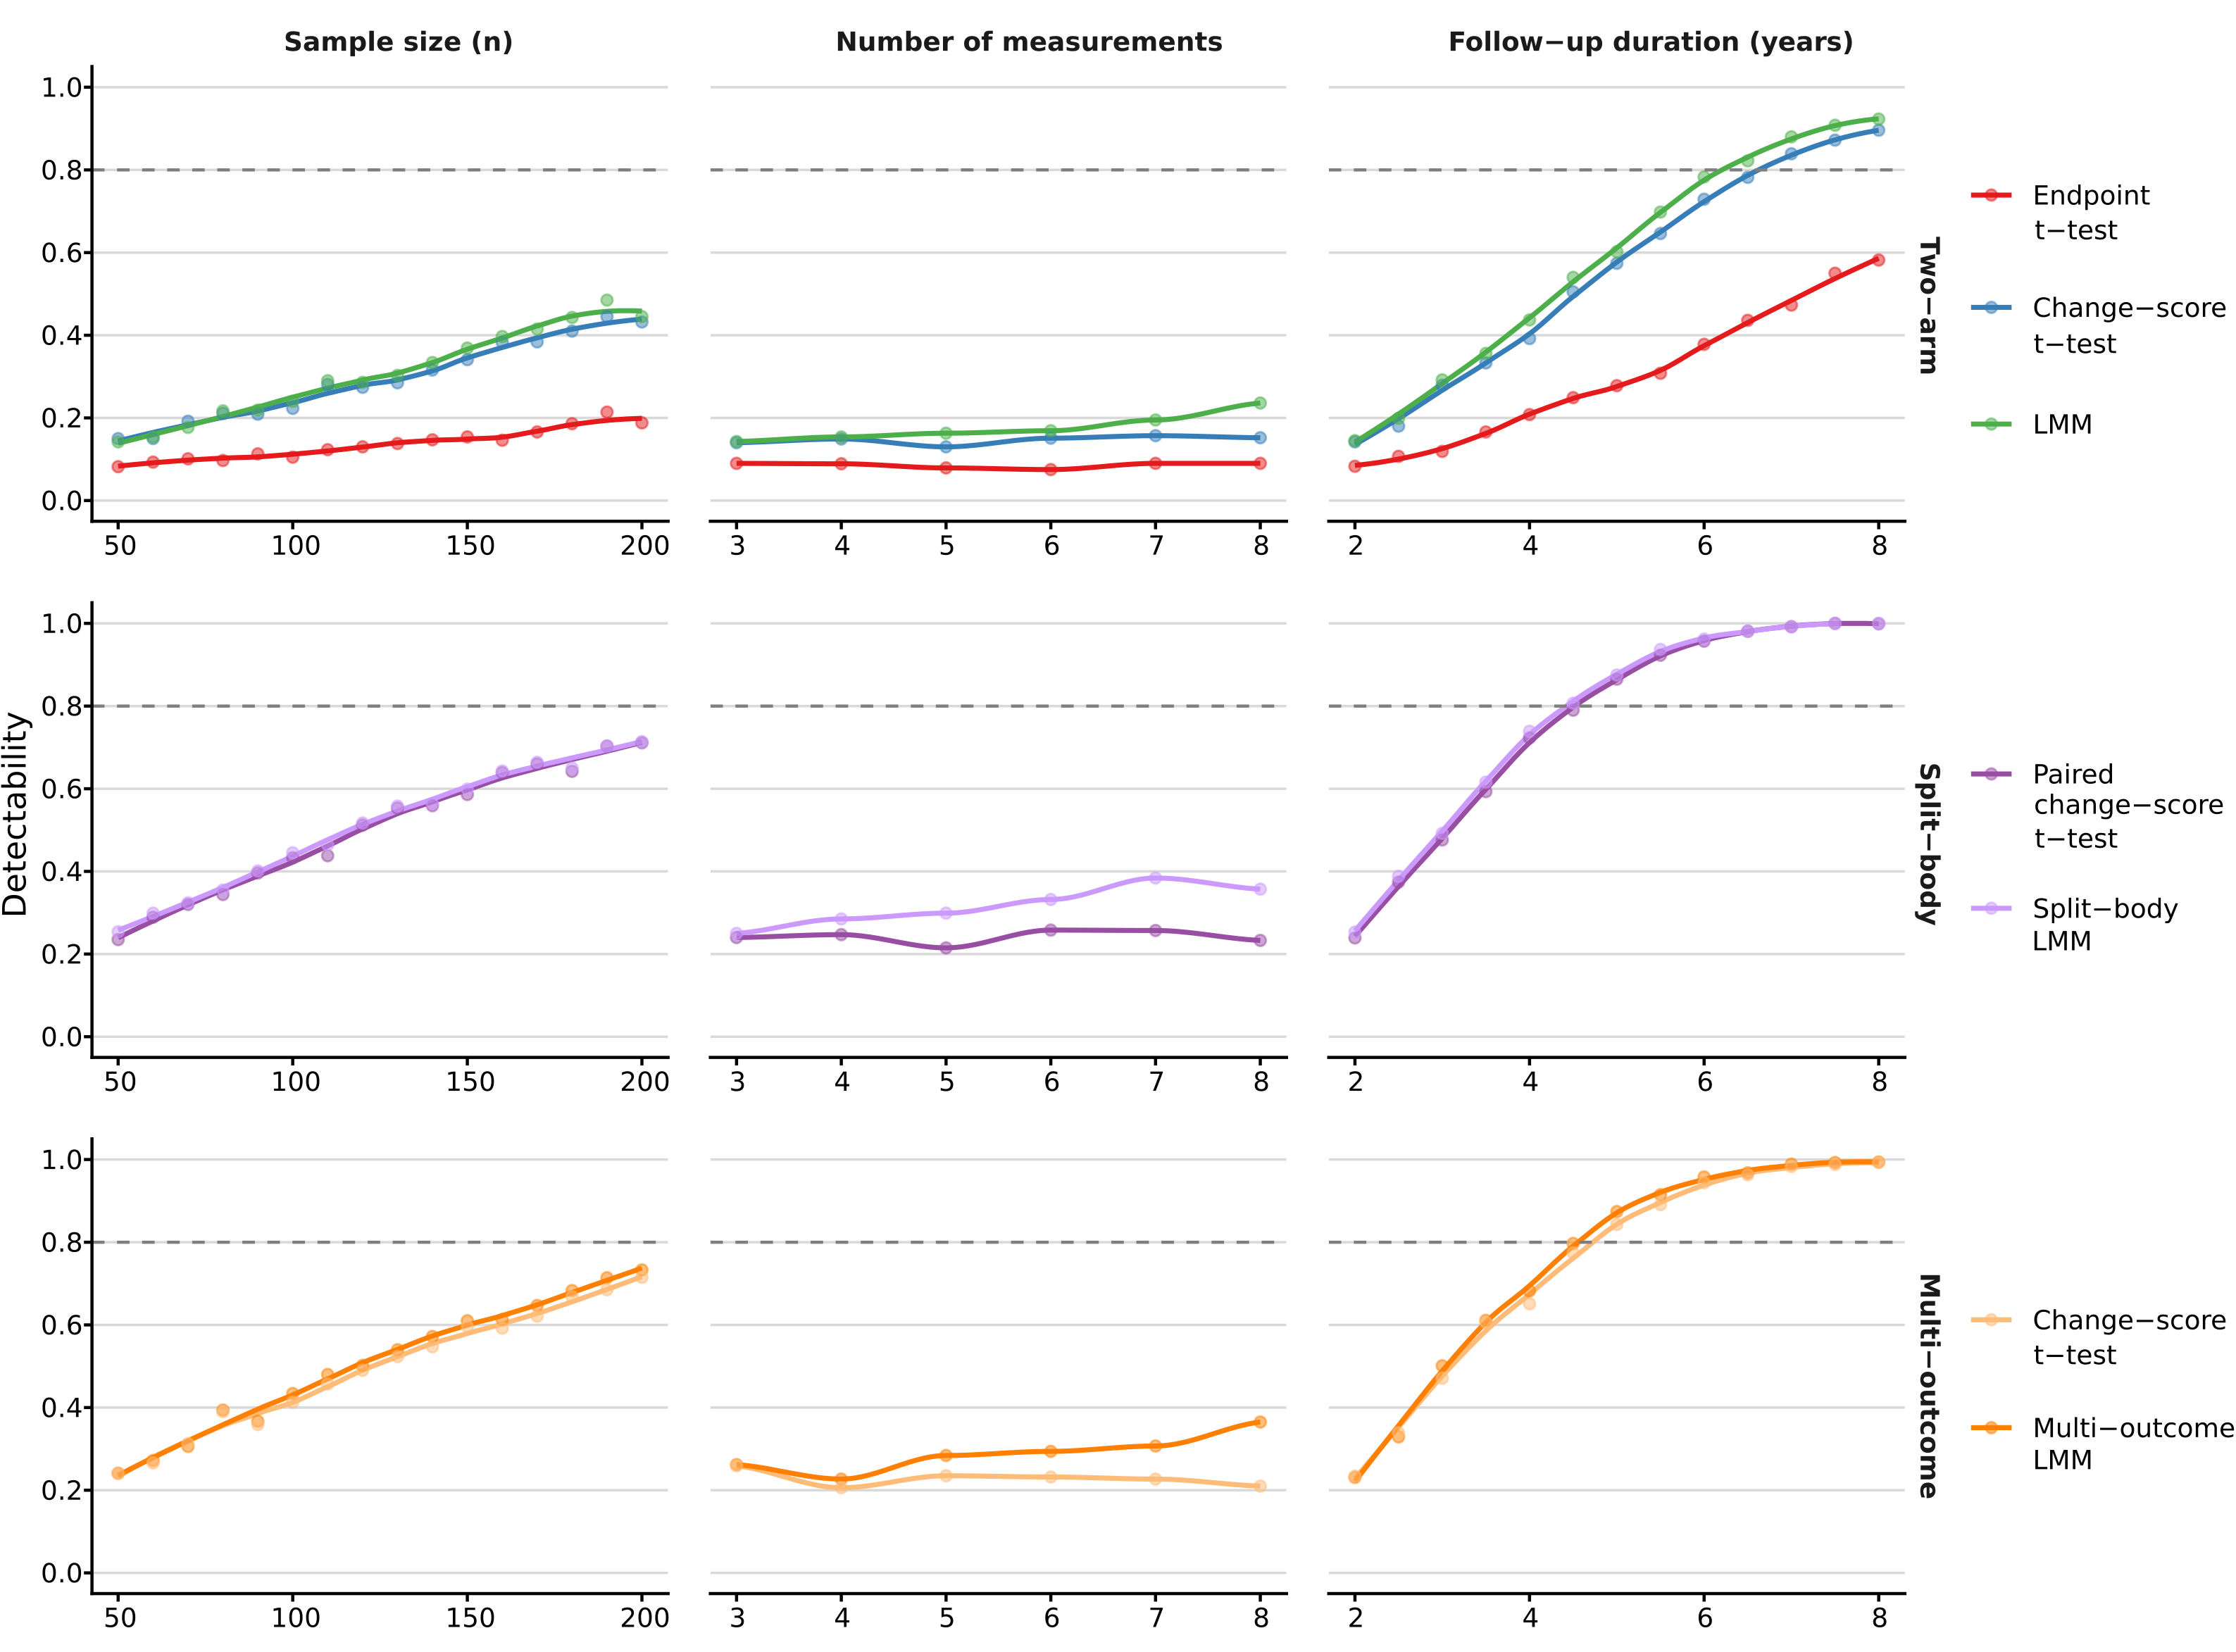
\includegraphics[width=1\linewidth]{figures/Figure_S1.png}
	\caption{\textbf{Detectability across study designs under higher within-individual variability.} As in Figure 3, but with within-individual variability set to $\sigma \approx 3.5$ kg. Each panel plots detectability, the proportion of simulated trials in which the intervention effect was detected at the $p < 0.05$ significance threshold, on the $y$-axis against a swept study-design parameter on the $x$-axis. Rows correspond to three study designs: two-arm between-individual (\textbf{top}), within-individual split-body (\textbf{middle}), and multi-outcome between-individual (\textbf{bottom}). Columns correspond to the parameter varied: sample size ($n$, 50--200; \textbf{left}), number of measurement occasions (3--8; \textbf{middle}), and follow-up duration (2--8 years; \textbf{right}). The higher variability lowers detectability across all designs but preserves the relative ordering of designs and analysis strategies.}
	\label{fig:figure_s1}
\end{figure*}

%%%%%%%%%%%%%%%%%%%%
% References Section
%%%%%%%%%%%%%%%%%%%%
\clearpage
\section{References}
\begingroup
\renewcommand{\section}[2]{}% suppress bibliography's internal \section*{References}
\fontsize{9pt}{10pt}\selectfont
\bibliographystyle{unsrtnat}
\bibliography{references}
\endgroup

\end{document}